\documentclass[12pt,a4paper]{article}
\usepackage[a4paper, margin=0.8in, headheight=14pt]{geometry}
\usepackage{fontspec}
\usepackage{unicode-math}
\setmainfont{TeX Gyre Pagella}
\setmonofont[Scale=0.88]{TeX Gyre Cursor}
\setmathfont{Latin Modern Math}
\usepackage{xcolor}
\usepackage{colortbl}
\usepackage{titlesec}
\usepackage{enumitem}
\usepackage{tabularx}
\usepackage{booktabs}
\usepackage{array}
\usepackage{amsmath}
\allowdisplaybreaks
\usepackage{tikz}
\usetikzlibrary{shapes.geometric, arrows.meta, positioning, calc, fit, decorations.pathreplacing, decorations.pathmorphing, patterns, backgrounds}
% circuitikz not required for this subject
\usepackage{tcolorbox}
\tcbuselibrary{skins, breakable}
\usepackage{etoolbox}
\usepackage{hyperref}
\usepackage{fancyhdr}
\usepackage{graphicx}
\usepackage{microtype}
\hyphenpenalty=10000
\exhyphenpenalty=10000
\sloppy
\usepackage{caption}
\usepackage{setspace}
\usepackage{multirow}
\usepackage{tocloft}
\newcommand{\Q}[1]{\textbf{#1}\par\noindent\ignorespaces}
\definecolor{myred}{RGB}{196,30,58}
\definecolor{mydark}{RGB}{30,30,50}
\definecolor{mygreen}{RGB}{14,120,80}
\definecolor{myteal}{RGB}{0,130,140}
\definecolor{myamber}{RGB}{180,100,0}
\definecolor{mypurple}{RGB}{100,30,160}
\definecolor{mygray}{RGB}{246,247,249}
\definecolor{mgframe}{RGB}{180,185,200}
\definecolor{watermark}{RGB}{145,150,170}
\definecolor{hdrred}{RGB}{250,232,235}
\definecolor{hdrgreen}{RGB}{220,244,233}
\definecolor{hdrteal}{RGB}{220,242,244}
\definecolor{hdramber}{RGB}{253,242,215}
\definecolor{hdrpurple}{RGB}{238,228,255}
\definecolor{hdrgray}{RGB}{238,240,245}
\definecolor{rowalt}{RGB}{250,251,253}
\AfterEndEnvironment{tcolorbox}{\color{mydark}}

\titleformat{\section}{\large\bfseries\color{myred}}{\thesection.}{0.5em}{}[\vspace{1pt}{\color{myred}\rule{\linewidth}{0.8pt}}]
\titleformat{\subsection}{\normalsize\bfseries\color{myteal}}{\thesubsection}{0.5em}{}
\titlespacing*{\section}{0pt}{18pt}{7pt}
\titlespacing*{\subsection}{0pt}{11pt}{4pt}
\setlength{\parindent}{0pt}
\setlength{\parskip}{4pt}
\renewcommand{\cfttoctitlefont}{\large\bfseries\color{myred}}
\renewcommand{\cftaftertoctitle}{\par\noindent{\color{myred}\rule{\linewidth}{0.8pt}}}
\setlength{\cftbeforetoctitleskip}{0pt}
\setlength{\cftaftertoctitleskip}{6pt}
\renewcommand{\cftsecfont}{\normalsize\bfseries\color{mydark}}
\renewcommand{\cftsecpagefont}{\normalsize\bfseries\color{mydark}}
\renewcommand{\cftsecleader}{\cftdotfill{\cftdotsep}}
\setlength{\cftbeforesecskip}{5pt}
\renewcommand{\cftsubsecfont}{\small\color{mydark}}
\renewcommand{\cftsubsecpagefont}{\small\color{mydark}}
\setlength{\cftbeforesubsecskip}{2pt}
\setlength{\cftsubsecindent}{1.4em}
\renewcommand{\cftpartfont}{\normalsize\bfseries\color{myteal}}
\renewcommand{\cftpartpagefont}{\normalsize\bfseries\color{myteal}}
\setlength{\cftbeforepartskip}{10pt}
\renewcommand{\arraystretch}{1.45}
\setlength{\tabcolsep}{6pt}
\arrayrulecolor{mydark}
\newcolumntype{B}[1]{>{\small\bfseries\raggedright\arraybackslash}m{#1}}
\newcolumntype{C}[1]{>{\centering\arraybackslash}m{#1}}
\newcolumntype{Y}{>{\small\raggedright\arraybackslash}X}
\renewcommand{\tabularxcolumn}[1]{m{#1}}
\newcommand{\currmodule}{Module 1}
\pagestyle{fancy}
\fancyhf{}
\fancyhead[L]{\small\color{myred}\textbf{EC501}\;\color{mydark}--- Electromagnetic Waves}
\fancyhead[R]{\small\color{myteal}\textbf{\currmodule\ Notes}}
\fancyfoot[C]{\small\color{mydark}\thepage}
\fancyfoot[R]{\small\color{watermark}\textit{\copyright\ Biraj}}
\renewcommand{\headrulewidth}{0.5pt}
\renewcommand{\footrulewidth}{0.3pt}

\hypersetup{colorlinks=true, linkcolor=myteal, urlcolor=myteal,
  pdfauthor={Biraj Sarkar},
  pdftitle={EC501 --- Combined Notes}}

\tcbset{
  tikzbox/.style={
    colback=mygray, colframe=mgframe, boxrule=0.6pt, arc=4pt,
    left=8pt, right=8pt, top=6pt, bottom=6pt,
    colbacktitle=mgframe, coltitle=mydark,
    fonttitle=\small\bfseries
  },
  defbox/.style={
    colback=hdrgreen, colframe=mygreen, boxrule=0.8pt, arc=4pt,
    left=9pt, right=9pt, top=6pt, bottom=6pt,
    colbacktitle=mygreen, coltitle=white,
    fonttitle=\small\bfseries
  },
  formulabox/.style={
    colback=hdrteal, colframe=myteal, boxrule=0.8pt, arc=4pt,
    left=9pt, right=9pt, top=7pt, bottom=7pt,
    colbacktitle=myteal, coltitle=white,
    fonttitle=\small\bfseries
  },
  examplebox/.style={
    colback=hdramber, colframe=myamber, boxrule=0.8pt, arc=4pt,
    left=9pt, right=9pt, top=6pt, bottom=6pt,
    colbacktitle=myamber, coltitle=white,
    fonttitle=\small\bfseries
  },
  masonbox/.style={
    colback=hdrpurple, colframe=mypurple, boxrule=0.8pt, arc=4pt,
    left=9pt, right=9pt, top=6pt, bottom=6pt,
    colbacktitle=mypurple, coltitle=white,
    fonttitle=\small\bfseries
  },
  exambox/.style={
    colback=hdrpurple, colframe=mypurple, boxrule=1pt, arc=5pt,
    left=10pt, right=10pt, top=8pt, bottom=8pt,
    colbacktitle=mypurple, coltitle=white,
    fonttitle=\bfseries,
    breakable, title after break={\textbf{Frequently Asked / Viva Questions (contd.)}}}
}
\tcbset{breakable}
\tcbset{coltext=mydark}
\tcbset{after={\color{mydark}}}

\tikzset{
  block/.style={rectangle, draw=myteal, fill=hdrteal,
    text width=2.4cm, align=center, minimum height=0.95cm,
    font=\small, rounded corners=3pt, line width=0.7pt},
  redblock/.style={rectangle, draw=myred, fill=hdrred,
    text width=2.4cm, align=center, minimum height=0.95cm,
    font=\small, rounded corners=3pt, line width=0.7pt},
  netnode/.style={rectangle, draw=myteal, fill=hdrteal,
    text width=1.5cm, align=center, minimum height=0.8cm,
    font=\small, rounded corners=3pt, line width=0.7pt},
  sumjunc/.style={circle, draw=myamber, fill=hdramber,
    minimum size=0.62cm, font=\small, line width=0.8pt},
  snode/.style={circle, draw=mypurple, fill=hdrpurple,
    minimum size=0.55cm, font=\footnotesize, line width=0.7pt},
  arrow/.style={-Stealth, thick, color=mydark},
  redarrow/.style={-Stealth, thick, color=myred},
  line/.style={thick, color=mydark}
}

\newcommand{\modulestart}[2]{%
  \clearpage
  \renewcommand{\currmodule}{Module #1}%
  \renewcommand{\theHsection}{mod#1.\arabic{section}}%
  \renewcommand{\theHsubsection}{\theHsection.\arabic{subsection}}%
  \renewcommand{\theHsubsubsection}{\theHsubsection.\arabic{subsubsection}}%
  \phantomsection
  \addcontentsline{toc}{part}{Module #1: #2}%
  \setcounter{section}{0}%
  \begin{center}
    \vspace*{1.0cm}
    {\Huge\bfseries\color{myred} Module #1}\\[10pt]
    {\Large\bfseries\color{mydark} #2}\\[10pt]
    {\color{myred}\rule{0.55\linewidth}{1.2pt}}
  \end{center}
  \vspace{14pt}
}
\begin{document}

\thispagestyle{empty}

% ─── Page Border (TikZ Overlay) ────────────────────────────────────────────────
\begin{tikzpicture}[remember picture, overlay]
  % Outer border (fine line in mgframe)
  \draw[color=mgframe, line width=1.5pt] 
    ($(current page.north west) + (0.6in, -0.6in)$) rectangle 
    ($(current page.south east) + (-0.6in, 0.6in)$);
  % Inner border (finer accent line in myred)
  \draw[color=myred, line width=0.8pt] 
    ($(current page.north west) + (0.65in, -0.65in)$) rectangle 
    ($(current page.south east) + (-0.65in, 0.65in)$);
\end{tikzpicture}

\vspace*{1.0cm}
\begin{center}
  {\Huge\bfseries\color{myred} EC501}\\[10pt]
  {\LARGE\bfseries\color{mydark} Electromagnetic Waves}\\[20pt]
  {\color{myred}\rule{0.7\linewidth}{1.5pt}}\\[18pt]
  {\Large\color{myteal}\textbf{Combined Module Notes}}\\[8pt]
  {\large\color{mydark} Modules 1 -- 5}\\[40pt]
  {\normalsize\color{mydark} Semester V \quad$\bullet$\quad ECE \quad$\bullet$\quad 3 Credits}\\[12pt]
  {\normalsize\color{mydark} CGEC \;$|$\; B.Tech ECE (2023--27)}
\end{center}
\vspace{1.0cm}
\begin{center}
  \begin{tcolorbox}[colback=mygray, colframe=mgframe, boxrule=0.5pt, arc=3pt, width=0.85\linewidth]
    \centering\small\color{mydark}
    \textbf{Disclaimer / Study Guide Notice:}\\
    These are condensed \textbf{Short Notes} focusing on core theory, key formulas, block/circuit diagrams, and standard viva Q\&As for university exam revision. Exhaustive numerical practice problems and derivation edge cases are not covered. This serves as a quick-revision reference guide for students.
  \end{tcolorbox}
\end{center}
\vfill
\vspace{0.6cm}
\begin{center}
  {\large\bfseries\color{mypurple} Biraj Sarkar}\\[16pt]
  {\footnotesize\color{watermark}\textbf{IN ASSOCIATION WITH}}\\[8pt]
  {\small\bfseries\color{mydark} MAKAUT Wingman \quad$\bullet$\quad MAKAUT Future Minds}\\[12pt]
  {\large\bfseries\color{myteal} Cooch Behar Government Engineering College}
\end{center}
\vfill
\begin{center}{\small\color{watermark}\textit{Exam-Ready Notes}}\end{center}
\clearpage

\hypersetup{linkcolor=mydark}
\tableofcontents
\hypersetup{linkcolor=myteal}
\clearpage

% -- Module 1 -----------------------------------------------------------------
\modulestart{1}{Vectors and Vector Calculus}

\section{Vectors and Vector Calculus}
\begin{tcolorbox}[defbox,title={Scalars, vectors and fields}]
A scalar has magnitude only. A vector has magnitude and direction. A field assigns a scalar or vector value to each point in a region.
\end{tcolorbox}
\begin{itemize}[leftmargin=*,itemsep=3pt]
\item \textbf{Components.} Write $\mathbf A=A_x\hat{\mathbf x}+A_y\hat{\mathbf y}+A_z\hat{\mathbf z}$. Its magnitude is $\sqrt{A_x^2+A_y^2+A_z^2}$ and its unit vector is $\mathbf A/|\mathbf A|$.
\item \textbf{Dot product.} $\mathbf A\cdot\mathbf B=\sum_i A_i B_i=|\mathbf A||\mathbf B|\cos\theta$. Use it for a projection or normal flux.
\item \textbf{Cross product.} The magnitude is $|\mathbf A||\mathbf B|\sin\theta$ with right-hand direction. Its $x$ component is $A_yB_z-A_zB_y$. Cycle $x,y,z$ for the others.
\item \textbf{Coordinates.} In cylindrical coordinates, $x=\rho\cos\phi$, $y=\rho\sin\phi$ and $dV=\rho\,d\rho\,d\phi\,dz$. In spherical coordinates, $\rho=r\sin\theta$, $z=r\cos\theta$ and $dV=r^2\sin\theta\,dr\,d\theta\,d\phi$. Here $\theta$ is measured from $+z$.
\end{itemize}
\subsection{Gradient, divergence and curl}
\begin{itemize}[leftmargin=*,itemsep=3pt]
\item \textbf{Gradient} $\nabla V$ gives the direction and rate of steepest increase of $V$. In Cartesian coordinates $\nabla=\hat{\mathbf x}\partial_x+\hat{\mathbf y}\partial_y+\hat{\mathbf z}\partial_z$.
\item \textbf{Divergence} $\nabla\cdot\mathbf A=\partial_xA_x+\partial_yA_y+\partial_zA_z$ gives net outward flux per volume. For a cylindrical radial field it reduces to $\rho^{-1}\partial_\rho(\rho A_\rho)$.
\item \textbf{Curl} $\nabla\times\mathbf A$ describes local circulation per area. Its $x$ component is $\partial_y A_z-\partial_z A_y$.
\item \textbf{Identities.} For smooth fields $\nabla\times\nabla V=0$, $\nabla\cdot(\nabla\times\mathbf A)=0$ and $\nabla^2V=\nabla\cdot\nabla V$.
\end{itemize}
\[
\begin{aligned}
\oint_{\partial V}\mathbf A\cdot d\mathbf S&=\int_V\nabla\cdot\mathbf A\,dV
 &&\text{(divergence theorem)},\\
\oint_{\partial S}\mathbf A\cdot d\boldsymbol\ell&=\int_S(\nabla\times\mathbf A)\cdot d\mathbf S
 &&\text{(Stokes' theorem)}.
\end{aligned}
\]
Use the outward normal on a closed surface and the right-hand rule for the boundary direction of an open surface.
For orthogonal coordinates $(u_1,u_2,u_3)$ let $h_i\,du_i$ denote the physical distance in direction $\hat{\mathbf u}_i$. The scale factors are $(1,\rho,1)$ for $(\rho,\phi,z)$ and $(1,r,r\sin\theta)$ for $(r,\theta,\phi)$. For cyclic indices $(i,j,k)$,
\[
\begin{aligned}
(\nabla V)_i &= \frac{\partial_i V}{h_i},\\
\nabla\cdot\mathbf A
 &= \frac{\sum_i \partial_i(h_jh_kA_i)}{h_1h_2h_3},\\
(\nabla\times\mathbf A)_i
 &=\frac{\partial_j(h_k A_k)-\partial_k(h_j A_j)}{h_jh_k}.
\end{aligned}
\]
For a spherical radial field $\mathbf A=A_r(r)\hat{\mathbf r}$, the divergence becomes $r^{-2}d(r^2 A_r)/dr$. This explains why an inverse-square radial field has zero divergence away from its source.
\begin{tcolorbox}[examplebox,title={Outward flux through a unit cube}]
For $\mathbf D=(2x,3y,4z)\,\mathrm{C/m^2}$ on $0\le x,y,z\le1$ metre, $\nabla\cdot\mathbf D=9\,\mathrm{C/m^3}$. Hence the flux is $9(1)=9\,\mathrm C$. Directly, the three zero-coordinate faces contribute zero and the opposite faces give $2+3+4=9\,\mathrm C$.
\end{tcolorbox}

\section{Basic Electromagnetic Laws}
\begin{tcolorbox}[defbox,title={Field quantities}]
$\mathbf E$ and $\mathbf H$ are field intensities in $\mathrm{V/m}$ and $\mathrm{A/m}$. $\mathbf D$ and $\mathbf B$ are flux densities in $\mathrm{C/m^2}$ and tesla. For a linear isotropic material, $\mathbf D=\epsilon\mathbf E$, $\mathbf B=\mu\mathbf H$ and $\mathbf J=\sigma\mathbf E$ for ohmic conduction.
\end{tcolorbox}
\begin{itemize}[leftmargin=*,itemsep=3pt]
\item \textbf{Coulomb law.} In a uniform dielectric a point charge gives $\mathbf E=q\hat{\mathbf r}/(4\pi\epsilon r^2)$. Add fields by superposition. The Lorentz force is $q(\mathbf E+\mathbf v\times\mathbf B)$.
\item \textbf{Gauss law and cylindrical symmetry.} An infinite line charge $\lambda_q$ in $\mathrm{C/m}$ gives $D_\rho(2\pi\rho L)=\lambda_q L$, so $E_\rho=\lambda_q/(2\pi\epsilon\rho)$.
\item \textbf{Electric potential.} For electrostatics $\mathbf E=-\nabla V$ and $V_b-V_a=-\int_a^b\mathbf E\cdot d\boldsymbol\ell$. In a uniform medium $\nabla^2V=-\rho_v/\epsilon$.
\item \textbf{Biot--Savart law.} A steady current element produces $d\mathbf H=I\,d\boldsymbol\ell'\times\hat{\mathbf R}/(4\pi R^2)$ with $\mathbf R$ directed from source to observer.
\item \textbf{Amp\`ere law for steady current.} A circular loop around an infinite straight wire gives $2\pi\rho H_\phi=I$. Direction follows the right-hand rule.
\end{itemize}
\begin{tcolorbox}[examplebox,title={Ampere law inside and outside a solid wire}]
A long wire of radius $a$ carries a steady current $I$ uniformly along $+z$. Choose an Amp\`erian circle of radius $\rho$ about the wire. Symmetry makes $H_\phi$ constant around it.
\[
\begin{aligned}
 2\pi\rho H_\phi&=I_{\rm enc},\\
 I_{\rm enc}&=I\rho^2/a^2 &&(0\le \rho\le a),\\
 I_{\rm enc}&=I &&(\rho\ge a).
\end{aligned}
\]
Hence $H_\phi=I\rho/(2\pi a^2)$ inside and $H_\phi=I/(2\pi\rho)$ outside, in $\mathrm{A/m}$. Both expressions agree at $\rho=a$. With $a=2\,\mathrm{mm}$ and $I=4\,\mathrm A$, $H_\phi$ is $159\,\mathrm{A/m}$ at $\rho=1\,\mathrm{mm}$ and also at $\rho=4\,\mathrm{mm}$. Use $B_\phi=\mu H_\phi$ if flux density is requested.
\end{tcolorbox}

\subsection{Maxwell equations in both forms}
\par\vspace{6pt}\noindent
\begin{tabularx}{\linewidth}{|B{3.3cm}|Y|Y|}\hline
Law & Integral form for fixed boundaries & Differential form \\ \hline
Electric Gauss & $\oint_S\mathbf D\cdot d\mathbf S=\int_V\rho_v\,dV$ & $\nabla\cdot\mathbf D=\rho_v$ \\ \hline
Magnetic Gauss & $\oint_S\mathbf B\cdot d\mathbf S=0$ & $\nabla\cdot\mathbf B=0$ \\ \hline
Faraday & $\oint_C\mathbf E\cdot d\boldsymbol\ell=-\frac{d}{dt}\int_S\mathbf B\cdot d\mathbf S$ & $\nabla\times\mathbf E=-\partial_t\mathbf B$ \\ \hline
Amp\`ere--Maxwell & $\oint_C\mathbf H\cdot d\boldsymbol\ell=\int_S(\mathbf J+\partial_t\mathbf D)\cdot d\mathbf S$ & $\nabla\times\mathbf H=\mathbf J+\partial_t\mathbf D$ \\ \hline
\end{tabularx}

Use the divergence theorem for flux laws and Stokes' theorem for circulation laws. The laws hold for arbitrary suitable regions, so equality of integrals gives equality of local densities. Faraday's minus sign expresses Lenz's law.
\begin{tcolorbox}[formulabox,title={Charge conservation and displacement current}]
\[
0=\nabla\cdot(\nabla\times\mathbf H)
 =\nabla\cdot\mathbf J+\partial_t(\nabla\cdot\mathbf D)
 \quad\Longrightarrow\quad \nabla\cdot\mathbf J=-\partial_t\rho_v .
\]
Displacement current density is $\partial_t\mathbf D$. Across an ideal capacitor gap, $A\partial_t D=dQ/dt$ accounts for the same current as flows in the leads. For phasors with time convention $e^{j\omega t}$, replace $\partial_t$ by $j\omega$.
\end{tcolorbox}

\begin{tcolorbox}[formulabox,title={Maxwell equations in a source-free lossless medium}]
For a homogeneous, linear, isotropic dielectric with no free charge or current and $\sigma=0$, put $\mathbf D=\epsilon\mathbf E$ and $\mathbf B=\mu\mathbf H$. For fields varying in time the four equations become
\[
\begin{aligned}
 \nabla\cdot\mathbf E&=0,& \nabla\cdot\mathbf H&=0,\\
 \nabla\times\mathbf E&=-\mu\partial_t\mathbf H,&
 \nabla\times\mathbf H&=\epsilon\partial_t\mathbf E .
\end{aligned}
\]
The last term remains even without conduction current. For sinusoidal fields write $j\omega$ in place of $\partial_t$. In SI, $\epsilon$ is in $\mathrm{F/m}$, $\mu$ in $\mathrm{H/m}$ and $\sigma$ in $\mathrm{S/m}$.
\end{tcolorbox}

% Reserve enough space for the section heading and its opening definition.
\par
\ifdim\dimexpr\pagegoal-\pagetotal\relax<115pt\relax
  \newpage
\fi
\section{Power Flow and Media Boundaries}
\subsection{Poynting theorem}
\begin{tcolorbox}[defbox,title={Poynting vector}]
The instantaneous Poynting vector $\mathbf S=\mathbf E\times\mathbf H$ gives electromagnetic power flux density in $\mathrm{W/m^2}$.
\end{tcolorbox}

For linear, nondispersive media, take the divergence of the cross product and substitute the two curl equations.
\[
\begin{aligned}
\nabla\cdot\mathbf S
 &= \mathbf H\cdot(\nabla\times\mathbf E)-\mathbf E\cdot(\nabla\times\mathbf H)\\
 &= -\mathbf H\cdot\partial_t\mathbf B-\mathbf E\cdot\partial_t\mathbf D-\mathbf J\cdot\mathbf E\\
 &= -\partial_t\left(\frac{\epsilon|\mathbf E|^2+\mu|\mathbf H|^2}{2}\right)
    -\mathbf J\cdot\mathbf E .
\end{aligned}
\]
After integration, inward power supplies the increase of stored field energy plus work done on currents. For an ohmic medium this last density is $\sigma|\mathbf E|^2$ in $\mathrm{W/m^3}$. With peak phasors, $\langle\mathbf S\rangle=\tfrac12\operatorname{Re}(\mathbf E\times\mathbf H^*)$. For $E=10\,\mathrm{V/m}$ and $H=10/377\,\mathrm{A/m}$ in phase and at right angles, average flux is $0.133\,\mathrm{W/m^2}$.
\subsection{Boundary conditions at a media interface}
\begin{tcolorbox}[tikzbox,title={Pillbox and narrow loop},unbreakable]
\centering
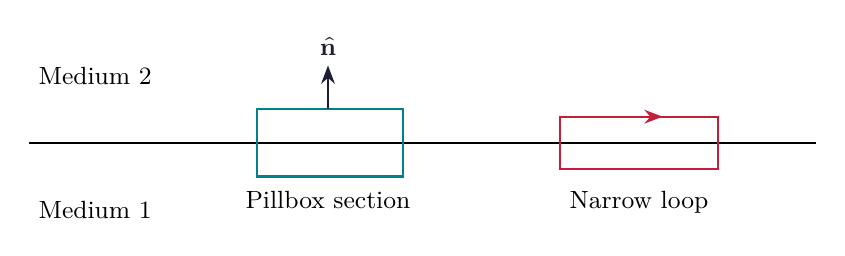
\begin{tikzpicture}[font=\small]
\draw[thick] (0,0)--(10,0);
\node[anchor=west] at (0,.85) {Medium 2};
\node[anchor=west] at (0,-.85) {Medium 1};
\draw[thick,myteal] (2.9,-.43) rectangle (4.75,.43);
\draw[arrow] (3.8,.43)--(3.8,.98) node[above] {$\hat{\mathbf n}$};
\node[below] at (3.8,-.49) {Pillbox section};
\draw[thick,myred] (6.75,-.33) rectangle (8.75,.33);
\draw[redarrow] (7.25,.33)--(8.05,.33);
\node[below] at (7.75,-.49) {Narrow loop};
\end{tikzpicture}
\end{tcolorbox}

Take $\hat{\mathbf n}$ from medium 1 to 2, free sheet charge $\rho_s$ in $\mathrm{C/m^2}$ and sheet current $\mathbf K_s$ in $\mathrm{A/m}$.
\begin{enumerate}[leftmargin=*,itemsep=3pt]
\item \textbf{Normal jumps.} Shrink the pillbox height so only cap flux remains. Opposite cap normals produce $\hat{\mathbf n}\cdot(\mathbf D_2-\mathbf D_1)=\rho_s$ and $\hat{\mathbf n}\cdot(\mathbf B_2-\mathbf B_1)=0$.
\item \textbf{Tangential jumps.} Take a loop of length $L$ along $\hat{\mathbf t}$ in medium 2 and back in medium 1. In Amp\`ere--Maxwell, as its height shrinks, $L(\mathbf H_2-\mathbf H_1)\cdot\hat{\mathbf t}=L\mathbf K_s\cdot(\hat{\mathbf n}\times\hat{\mathbf t})$. This gives $\hat{\mathbf n}\times(\mathbf H_2-\mathbf H_1)=\mathbf K_s$. In Faraday's law the flux term vanishes with the loop area, so $\hat{\mathbf n}\times(\mathbf E_2-\mathbf E_1)=0$.
\item \textbf{Perfect electric conductor (PEC).} Take zero time-harmonic fields inside and a normal pointing out of the conductor. Outside, $\mathbf E_t=0$, $B_n=0$, $D_n=\rho_s$ and $\hat{\mathbf n}\times\mathbf H=\mathbf K_s$.
\end{enumerate}

\begin{tcolorbox}[examplebox,title={Normal and tangential electric fields}]
At $z=0$, $\epsilon_1=2\epsilon_0$, $\epsilon_2=5\epsilon_0$ and $\rho_s=0$. For $\mathbf E_1=3\hat{\mathbf x}+4\hat{\mathbf z}\,\mathrm{V/m}$, $E_{2x}=E_{1x}=3\,\mathrm{V/m}$ but $E_{2z}=(\epsilon_1/\epsilon_2)E_{1z}=1.6\,\mathrm{V/m}$. It is the normal $\mathbf D$ that remains continuous.
\end{tcolorbox}

\newpage
\begin{center}
  {\large\bfseries\color{myred} Quick Revision --- Module 1}\\[3pt]
  {\small\color{mydark} Vectors, Maxwell Equations and Boundaries $|$ EC501}
\end{center}
\noindent{\color{myred}\rule{\linewidth}{1.2pt}}
\begin{tcolorbox}[formulabox,title={Key Formulas at a Glance}]
\renewcommand{\arraystretch}{1.35}
\begin{tabularx}{\linewidth}{B{5.0cm}Y}
Gauss laws & $\nabla\cdot\mathbf D=\rho_v$, $\nabla\cdot\mathbf B=0$ \\[3pt]
Faraday & $\nabla\times\mathbf E=-\partial_t\mathbf B$ \\[3pt]
Amp\`ere--Maxwell & $\nabla\times\mathbf H=\mathbf J+\partial_t\mathbf D$ \\[3pt]
Continuity & $\nabla\cdot\mathbf J=-\partial_t\rho_v$ \\[3pt]
Average flux & $\tfrac12\operatorname{Re}(\mathbf E\times\mathbf H^*)$ for peak phasors \\[3pt]
\end{tabularx}
\end{tcolorbox}
\begin{tcolorbox}[defbox,title={One-Line Definitions}]
\textbf{Gradient.} Vector pointing in the direction of steepest increase of a scalar.\par
\textbf{Displacement current density.} Time derivative of electric flux density.\par
\textbf{Poynting vector.} Directed electromagnetic power transmitted per unit area.\par
\end{tcolorbox}
\begin{tcolorbox}[exambox,title={Frequently Asked / Viva Questions}]
\begin{enumerate}[topsep=0pt, label=\textbf{Q\arabic*.}, itemsep=5pt]
\item \Q{What is the divergence theorem used for?}
Convert closed-surface outward flux to a volume integral.
\item \Q{What is the use of Stokes' theorem?}
Convert loop circulation to a surface integral of curl.
\item \Q{What is zero in magnetic Gauss law?}
Net magnetic flux through a closed surface.
\item \Q{What does Faraday's minus sign mean?}
Induction has a direction that opposes the flux change.
\item \Q{What crosses an ideal capacitor gap?}
Displacement current $dQ/dt$, associated with the changing field.
\item \Q{How is charge continuity obtained?}
Take divergence of Amp\`ere--Maxwell and use electric Gauss law.
\item \Q{Why is the magnetic phasor conjugated in average power?}
Averaging the real fields retains their relative phase.
\item \Q{What jumps across a sheet with free charge?}
The normal component of $\mathbf D$, by $\rho_s$.
\item \Q{What causes a tangential magnetic field jump?}
A free surface current $\mathbf K_s$.
\item \Q{Which electric component is zero at a PEC wall?}
The tangential component at its surface.
\end{enumerate}
\end{tcolorbox}
\begin{tcolorbox}[tikzbox,title={Summary comparison}]
\begin{tabularx}{\linewidth}{|B{4cm}|Y|}\hline
\textbf{Case} & \textbf{What to use} \\ \hline
Pillbox & Normal $\mathbf D$ and $\mathbf B$. \\ \hline
Narrow loop & Tangential $\mathbf E$ and $\mathbf H$. \\ \hline
Energy balance & Inward flux supplies stored energy increase and work on currents. \\ \hline
\end{tabularx}
\end{tcolorbox}

% -- Module 2 -----------------------------------------------------------------
\modulestart{2}{Uniform Plane Waves}

\section{Uniform Plane Waves}
\begin{tcolorbox}[defbox,title={Uniform plane wave}]
A uniform plane wave has the same field at every point in a plane perpendicular to propagation. In a source-free homogeneous isotropic medium the electric and magnetic fields are transverse.
\end{tcolorbox}
\subsection{Wave equation and travelling fields}
Use peak phasors with $e^{j\omega t}$ and real material constants $\mu,\epsilon,\sigma$. In a source-free bulk medium, $\nabla\cdot\mathbf E=0$. Taking curl of Faraday's law gives
\[
\begin{aligned}
\nabla\times\nabla\times\mathbf E
 &=-j\omega\mu(\sigma+j\omega\epsilon)\mathbf E,\\
\nabla^2\mathbf E&=\gamma^2\mathbf E,\qquad
\gamma=\sqrt{j\omega\mu(\sigma+j\omega\epsilon)}=\alpha+j\beta .
\end{aligned}
\]
Curling Amp\`ere--Maxwell in the same homogeneous medium gives $\nabla^2\mathbf H=\gamma^2\mathbf H$ using $\nabla\cdot\mathbf H=0$. In time domain the electric-field equation is
\[
 \nabla^2\mathbf E=\mu\sigma\,\partial_t\mathbf E+
                      \mu\epsilon\,\partial_t^2\mathbf E.
\]
The first term accounts for conduction and the second for displacement current.
The decaying forward solution is $\mathbf E=\mathbf E_0e^{-\gamma\hat{\mathbf k}\cdot\mathbf r}$. Use $\nabla\times\mathbf E=-\gamma\hat{\mathbf k}\times\mathbf E$ to obtain $\mathbf H=\hat{\mathbf k}\times\mathbf E/\eta$, where $\eta=j\omega\mu/\gamma$ in ohms.
\begin{itemize}[leftmargin=*,itemsep=3pt]
\item \textbf{Lossless limit.} $\alpha=0$, $\beta=k=\omega\sqrt{\mu\epsilon}$ and $\eta=\sqrt{\mu/\epsilon}$. In free space $v=1/\sqrt{\mu_0\epsilon_0}\approx 3\times10^8\,\mathrm{m/s}$ and $\eta_0\approx377\,\Omega$.
\item \textbf{Phase velocity.} Keeping $\omega t-\beta z$ constant gives $v_p=\omega/\beta=f\lambda$. Here $\lambda=2\pi/\beta$.
\item \textbf{Group velocity.} Superpose nearby frequencies and write the envelope phase as $\Delta\omega\,t-\Delta\beta\,z$. The envelope moves at $v_g=d\omega/d\beta$ for a narrow band with weak distortion. For $\beta$ proportional to $\omega$, $v_g=v_p$. With strong loss or dispersion, a reshaped pulse peak need not track energy.
\end{itemize}

\subsection{Polarization and the Poincar\'e sphere}
\begin{tcolorbox}[defbox,title={Polarization}]
Polarization describes the trajectory and sense traced by the tip of the electric field at a fixed point. Only the relative amplitudes and phases of the transverse components matter.
\end{tcolorbox}

For propagation along $+z$, use $\mathbf E=(a\hat{\mathbf x}+be^{j\Delta}\hat{\mathbf y})e^{-jkz}$ with $a,b\ge0$. At fixed $z$ write $u=E_x/a$ and $v=E_y/b$. Eliminating the common time phase from $u=\cos\psi$ and $v=\cos(\psi+\Delta)$ gives
\[
u^2+v^2-2uv\cos\Delta=\sin^2\Delta .
\]
\begin{itemize}[leftmargin=*,itemsep=3pt]
\item \textbf{Linear.} Relative phase $0$ or $\pi$, or one component zero. The field moves along a fixed line.
\item \textbf{Circular.} Equal magnitudes and $\Delta=\pm\pi/2$. For $\Delta=-\pi/2$ the field initially moves from $+x$ towards $+y$. State the viewing direction if giving a handedness name.
\item \textbf{Elliptical.} The general nondegenerate case. Axial ratio is major semiaxis divided by minor semiaxis, so it equals 1 for a circle and tends to infinity for a line.
\end{itemize}
For a fully polarized wave, the normalized Stokes coordinates $s_i=S_i/S_0$ give a point on the unit Poincar\'e sphere:
\[
\begin{aligned}
S_0 &= a^2+b^2,&S_1 &=a^2-b^2,\\
S_2 &=2ab\cos\Delta,& S_3 &=2ab\sin\Delta .
\end{aligned}
\]
This choice defines the pole signs. Verify $S_1^2+S_2^2+S_3^2=S_0^2$ by squaring. The ellipse tilt is $\tfrac12\operatorname{atan2}(s_2,s_1)$ and signed ellipticity angle is $\chi=\tfrac12\sin^{-1}(s_3)$. The axial ratio is $1/|\tan\chi|$. At the poles the tilt is undefined. The equator is linear, poles are circular, and antipodal points represent orthogonal states.
\begin{tcolorbox}[tikzbox,title={Poincar\'e sphere for the stated Stokes convention},unbreakable]
\centering
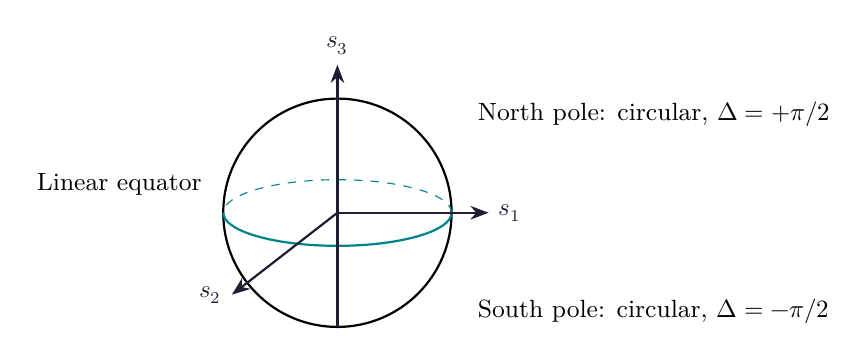
\begin{tikzpicture}[font=\small]
\draw[thick] (0,0) circle (1.45);
\draw[dashed,myteal] (1.45,0) arc (0:180:1.45 and .42);
\draw[myteal,thick] (-1.45,0) arc (180:360:1.45 and .42);
\draw[arrow] (0,-1.45)--(0,1.88) node[above] {$s_3$};
\draw[arrow] (0,0)--(1.92,0) node[right] {$s_1$};
\draw[arrow] (0,0)--(-1.34,-1.04) node[left] {$s_2$};
\node[anchor=west] at (1.66,1.25) {North pole: circular, $\Delta=+\pi/2$};
\node[anchor=west] at (1.66,-1.25) {South pole: circular, $\Delta=-\pi/2$};
\node[anchor=east] at (-1.6,.36) {Linear equator};
\end{tikzpicture}
\end{tcolorbox}

For $(E_x,E_y)=(3,-j)\,\mathrm{V/m}$, the axes are $x,y$ and axial ratio is 3. The normalized point is $(8/10,0,-6/10)$.

\section{Propagation in Conducting Media}
\begin{tcolorbox}[defbox,title={Skin depth}]
Skin depth $\delta=1/\alpha$ is the distance over which a plane-wave field amplitude falls to $1/e$ of its surface value.
\end{tcolorbox}

Squaring $\gamma=\alpha+j\beta$ gives $\beta^2-\alpha^2=\omega^2\mu\epsilon$ and $2\alpha\beta=\omega\mu\sigma$. Squaring and adding gives $\beta^2+\alpha^2=\omega^2\mu\epsilon\sqrt{1+(\sigma/\omega\epsilon)^2}$. Thus, with $t=\sigma/(\omega\epsilon)$,
\[
\alpha=\omega\sqrt{\frac{\mu\epsilon}{2}(\sqrt{1+t^2}-1)},\qquad
\beta=\omega\sqrt{\frac{\mu\epsilon}{2}(\sqrt{1+t^2}+1)} .
\]
\begin{itemize}[leftmargin=*,itemsep=3pt]
\item \textbf{Low-loss dielectric} ($t\ll1$). $\beta\approx\omega\sqrt{\mu\epsilon}$ and $\alpha\approx(\sigma/2)\sqrt{\mu/\epsilon}$.
\item \textbf{Good conductor} ($t\gg1$). $\gamma\approx(1+j)\sqrt{\omega\mu\sigma/2}$, $\delta\approx\sqrt{2/(\omega\mu\sigma)}$ and $\eta\approx(1+j)R_s$ where $R_s=1/(\sigma\delta)$ in $\Omega$ per square.
\item \textbf{Current and power.} For a thick, locally flat conductor, inward depth $u$ gives $\mathbf J_t(u)=\sigma\mathbf E_t(0)e^{-(1+j)u/\delta}$. Integrating gives equivalent sheet current $\mathbf K=\sigma\mathbf E_t(0)/\gamma$. The metal-to-outside normal gives $\mathbf K\approx\hat{\mathbf n}\times\mathbf H_t$.
\end{itemize}
The ratio $t$ compares the magnitudes of conduction and displacement current densities. A perfect dielectric has $t=0$. A lossy dielectric has nonzero conductivity in this model, and the low-loss approximation requires $t\ll1$. Around $t=1$ use both terms. For instance, a material with $\epsilon_r=12$ and $\sigma=0.001\,\mathrm{S/m}$ has $t\approx0.30$ at $5\,\mathrm{MHz}$. With $\epsilon_r=60$ and $\sigma=1.2\,\mathrm{S/m}$ at the same frequency, $t\approx72$ and the good-conductor approximation is appropriate.

With peak phasors, the mean loss per unit area is
\[
\begin{aligned}
p_s&=\int_0^\infty \tfrac12\sigma|\mathbf E_t(0)|^2 e^{-2u/\delta}\,du\\
   &=\frac{\sigma\delta}{4}|\mathbf E_t(0)|^2
    =\tfrac12 R_s |\mathbf H_t(0)|^2 .
\end{aligned}
\]
\begin{tcolorbox}[examplebox,title={Skin depth and heating in copper}]
At $10\,\mathrm{MHz}$ take $\mu=\mu_0$ and $\sigma=5.8\times10^7\,\mathrm{S/m}$. Then $\delta\approx20.9\,\mu\mathrm m$ and $R_s\approx0.825\,\mathrm{m}\Omega$. At $|\mathbf H_t|=10\,\mathrm{A/m}$ peak, $p_s\approx0.0413\,\mathrm{W/m^2}$.
\end{tcolorbox}

\begin{tcolorbox}[examplebox,title={Extract wave parameters from attenuation data}]
At $20\,\mathrm{MHz}$ a wave has $\beta=2.4\,\mathrm{rad/m}$ and retains $25\%$ of its field amplitude after $3\,\mathrm m$. Use $|E(z)|/|E(0)|=e^{-\alpha z}$.
\[
\begin{aligned}
 \alpha&=-\ln(0.25)/3=0.462\,\mathrm{Np/m},\\
 \delta&=1/\alpha=2.16\,\mathrm m,\\
 v_p&=2\pi f/\beta=5.24\times10^7\,\mathrm{m/s}.
\end{aligned}
\]
For this uniform forward wave the power fraction is $e^{-2\alpha z}$. A statement that $25\%$ of the \emph{power} remains would give half the above attenuation constant.
\end{tcolorbox}

\section{Plane Waves at a Media Interface}
\subsection{Arbitrary direction, reflection and refraction}
At $z=0$ take incidence from medium 1 ($z<0$) into medium 2. Rotate the axes so the plane of incidence is $xz$. An arbitrary incident direction then has $\mathbf k_i=k_1(\hat{\mathbf x}\sin\theta_i+\hat{\mathbf z}\cos\theta_i)$ and a phase factor $e^{-j\mathbf k_i\cdot\mathbf r}$ in a lossless medium. Tangential phase factors must match at every point on the interface. Therefore
\[
 k_1\sin\theta_i=k_1\sin\theta_r=k_2\sin\theta_t .
\]
This gives $\theta_r=\theta_i$ and Snell's law. For isotropic dielectrics use $n_1\sin\theta_i=n_2\sin\theta_t$, where $n_m=ck_m/\omega$.
\begin{tcolorbox}[tikzbox,title={Oblique incidence and tangential phase matching},unbreakable]
\centering
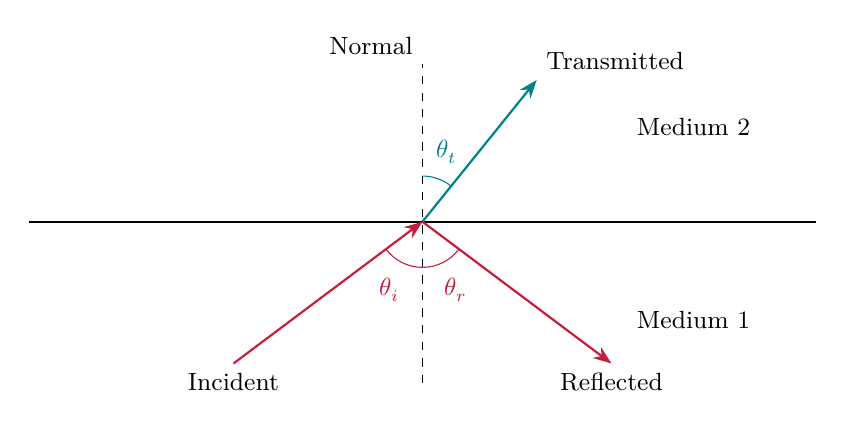
\begin{tikzpicture}[font=\small]
\draw[thick] (-5,0)--(5,0);
\draw[dashed] (0,-2.05)--(0,2.0) node[above left] {Normal};
\draw[redarrow] (-2.4,-1.8)--(0,0);
\draw[redarrow] (0,0)--(2.4,-1.8);
\draw[arrow,color=myteal] (0,0)--(1.45,1.8);
\node[anchor=west] at (2.6,1.2) {Medium 2};
\node[anchor=west] at (2.6,-1.25) {Medium 1};
\node[below] at (-2.4,-1.8) {Incident};
\node[below] at (2.4,-1.8) {Reflected};
\node[above right] at (1.45,1.8) {Transmitted};
\draw[myred] (0,-.58) arc[start angle=270,end angle=217,radius=.58];
\draw[myred] (0,-.58) arc[start angle=270,end angle=323,radius=.58];
\draw[myteal] (0,.58) arc[start angle=90,end angle=51,radius=.58];
\node[myred] at (-.42,-.86) {$\theta_i$};
\node[myred] at (.42,-.86) {$\theta_r$};
\node[myteal] at (.31,.89) {$\theta_t$};
\end{tikzpicture}
\end{tcolorbox}
\subsection{TE, TM and Fresnel coefficients}
Transverse electric (TE or s) has $\mathbf E$ perpendicular to the incidence plane. Transverse magnetic (TM or p) has $\mathbf H$ perpendicular to that plane. Define $E_i,E_r,E_t$ as signed \emph{tangential electric} components along the same coordinate direction in all three waves. For one forward component the wave admittance is $Y_{\mathrm{TE}}=\cos\theta/\eta$ and $Y_{\mathrm{TM}}=1/(\eta\cos\theta)$, obtained by resolving $\mathbf H=\hat{\mathbf k}\times\mathbf E/\eta$.
\[
\begin{aligned}
E_i+E_r &= E_t,&
Y_1(E_i-E_r)&=Y_2E_t,\\
r=\frac{E_r}{E_i}&=\frac{Y_1-Y_2}{Y_1+Y_2},&
t_E=\frac{E_t}{E_i}&=1+r=\frac{2Y_1}{Y_1+Y_2}.
\end{aligned}
\]
\begin{itemize}[leftmargin=*,itemsep=3pt]
\item \textbf{Normal incidence.} Both polarizations give $r=(\eta_2-\eta_1)/(\eta_1+\eta_2)$. At oblique incidence $t_E$ for TM refers to tangential components, so the total field ratio adds a factor $\cos\theta_i/\cos\theta_t$.
\item \textbf{Power ratios.} The normal flux is $\tfrac12\operatorname{Re}(Y)|E_{\tan}|^2$ for a forward wave. For a lossless incident medium, $R=|r|^2$ and $T=\operatorname{Re}(Y_2)|t_E|^2/Y_1$. At an ordinary lossless interface $R+T=1$.
\item \textbf{Brewster angle.} For equal permeabilities and different real refractive indices, TM reflection vanishes when $Y_{1,\mathrm{TM}}=Y_{2,\mathrm{TM}}$. Substituting $\eta_m\propto1/n_m$ and Snell's law gives $\theta_i+\theta_t=90^\circ$, hence $\tan\theta_B=n_2/n_1$. Reflected light can therefore be purely TE.
\item \textbf{Polarization change.} Decompose the incident field into TE and TM and apply each coefficient separately. Unequal magnitudes alter the orientation and axial ratio. A relative phase change, such as in total internal reflection, can turn linear polarization into elliptical.
\end{itemize}
\begin{tcolorbox}[examplebox,title={Compare TE and TM power reflection at oblique incidence}]
From air onto a lossless nonmagnetic dielectric with $n_2=2$, let $\theta_i=30^\circ$. Snell gives $\sin\theta_t=0.25$ and $\cos\theta_t=0.9682$. Use $\eta_2=\eta_0/2$.
\[
\begin{aligned}
 r_{\mathrm{TE}}&=\frac{0.8660-1.9365}{0.8660+1.9365}
                  =-0.382,& R_{\mathrm{TE}}&=0.146,\\
 r_{\mathrm{TM}}&=\frac{1.1547-2.0656}{1.1547+2.0656}
                  =-0.283,& R_{\mathrm{TM}}&=0.080.
\end{aligned}
\]
The numerators use the tangential-electric convention and both admittances are scaled by $\eta_0$. Power transmittance is $1-R$ for each polarization. The negative field sign gives phase reversal, not negative reflected power.
\end{tcolorbox}

\subsection{Total internal reflection and conducting boundary}
For $n_1>n_2$ the critical angle is $\theta_c=\sin^{-1}(n_2/n_1)$. Above it $k_x>k_2$ and $k_{2z}=-j\kappa$ with $\kappa=\sqrt{k_x^2-k_2^2}$ for decay into $z>0$. The transmitted field varies as $e^{-jk_x x}e^{-\kappa z}$. It is evanescent and has zero mean normal power in a lossless second half-space. The reflected magnitude is unity but its phase can differ between TE and TM.
\begin{tcolorbox}[examplebox,title={Glass to air and air to glass}]
Glass-to-air with $n_1=1.5$, $n_2=1$ gives $\theta_c=\sin^{-1}(1/1.5)=41.8^\circ$. At $50^\circ$, $k_x=1.149k_0$ and $\kappa=0.566k_0$. In the reverse direction at normal incidence, $r=(377/1.5-377)/(377/1.5+377)=-0.2$. Power reflection is $4\%$ and transmission is $96\%$.
\end{tcolorbox}

For a perfect electric conductor, $\mathbf E_{\tan}=0$ so $r=-1$ for tangential electric field. At normal incidence onto $z=0$ from $z<0$,
\[
 E_x=-2jE_0\sin(kz),\qquad H_y=2(E_0/\eta)\cos(kz).
\]
The wall is an electric node and a magnetic antinode, and mean normal power is zero. For a finite good conductor, use its complex $\eta$ at normal incidence. The reflected amplitude is below unity and the transmitted normal power is dissipated over the skin layer.
At oblique PEC incidence the reflected tangential electric component again has opposite sign. Let $\psi=e^{-jk_x x}$ and let $E_i$ be the tangential electric amplitude at the wall reference plane. Then $E_{\tan}=-2j E_i\psi\sin(k_z z)$. For TE this is the entire electric field. For TM use $\mathbf k\cdot\mathbf E=0$ separately for each wave to get $E_z=-2(k_x/k_z) E_i\psi\cos(k_z z)$. Normal electric field at the wall is allowed and is supported by surface charge. The tangential magnetic fields add at the wall and support surface current.

\newpage
\begin{center}
  {\large\bfseries\color{myred} Quick Revision --- Module 2}\\[3pt]
  {\small\color{mydark} Uniform Plane Waves and Media Interfaces $|$ EC501}
\end{center}
\noindent{\color{myred}\rule{\linewidth}{1.2pt}}
\begin{tcolorbox}[formulabox,title={Key Formulas at a Glance}]
\renewcommand{\arraystretch}{1.35}
\begin{tabularx}{\linewidth}{B{5.0cm}Y}
Propagation & $\gamma^2=j\omega\mu(\sigma+j\omega\epsilon)$ \\[3pt]
Speed & $v_p=\omega/\beta$, $v_g=d\omega/d\beta$ \\[3pt]
Skin depth & $\delta=1/\alpha\approx\sqrt{2/(\omega\mu\sigma)}$ in a good conductor \\[3pt]
Phase matching & $n_1\sin\theta_i=n_2\sin\theta_t$ \\[3pt]
Fresnel coefficient & $r=(Y_1-Y_2)/(Y_1+Y_2)$ for tangential electric field \\[3pt]
Total internal reflection & $\theta_c=\sin^{-1}(n_2/n_1)$ for $n_1>n_2$ \\[3pt]
\end{tabularx}
\end{tcolorbox}
\begin{tcolorbox}[defbox,title={One-Line Definitions}]
\textbf{Wave impedance.} Ratio of transverse electric to magnetic magnitudes as a complex field ratio, in ohms.\par
\textbf{Polarization.} Locus and rotation sense of the electric vector at a fixed point.\par
\textbf{Evanescent field.} A field whose amplitude decays exponentially in a spatial direction.\par
\end{tcolorbox}
\begin{tcolorbox}[exambox,title={Frequently Asked / Viva Questions}]
\begin{enumerate}[topsep=0pt, label=\textbf{Q\arabic*.}, itemsep=5pt]
\item \Q{What is uniform on a plane-wave wavefront?}
The field across a plane normal to propagation.
\item \Q{When is a transverse wave circular?}
Equal orthogonal amplitudes in phase quadrature.
\item \Q{What is plotted on the Poincar\'e sphere?}
The three normalized Stokes coordinates.
\item \Q{What distinguishes phase and group velocity?}
One follows a phase point and the other follows a narrow-band envelope.
\item \Q{Why does copper carry high-frequency current near its surface?}
Its high conductivity gives a large attenuation constant and small skin depth.
\item \Q{What is the surface-loss density for a peak field?}
$\tfrac12R_s|\mathbf H_t|^2$.
\item \Q{Why must tangential wave number match?}
The boundary conditions must hold at all points of the interface.
\item \Q{Which dielectric reflection vanishes at Brewster incidence?}
TM for lossless dielectrics of equal permeability.
\item \Q{What remains in the second medium above the critical angle?}
A decaying field with zero mean normal flux in a lossless half-space.
\item \Q{What is the PEC electric reflection coefficient?}
Minus one for the tangential electric component.
\end{enumerate}
\end{tcolorbox}
\begin{tcolorbox}[tikzbox,title={Summary comparison}]
\begin{tabularx}{\linewidth}{|B{4cm}|Y|}\hline
\textbf{Case} & \textbf{What to use} \\ \hline
Lossless plane wave & Real $\eta$ and no attenuation. \\ \hline
Good conductor & $\alpha\approx\beta$, with $\eta\approx(1+j)R_s$. \\ \hline
TE / TM & $Y=\cos\theta/\eta$ for TE, $Y=1/(\eta\cos\theta)$ for TM. \\ \hline
\end{tabularx}
\end{tcolorbox}

% -- Module 3 -----------------------------------------------------------------
\modulestart{3}{Distributed Transmission-Line Model}

\section{Distributed Transmission-Line Model}
\begin{tcolorbox}[defbox,title={Transmission line}]
A transmission line is a distributed structure guiding electromagnetic energy. Voltage and current depend on position. The distributed model matters when propagation delay is comparable to a signal's time scale or the length is a significant fraction of wavelength.
\end{tcolorbox}

With current referenced toward the load along $+z$, a length $\Delta z$ has series $R\Delta z$, $L\Delta z$ and shunt $G\Delta z$, $C\Delta z$. Here $R,L,G,C$ denote resistance, inductance, conductance and capacitance per metre. Use peak phasors and $e^{j\omega t}$.
\begin{tcolorbox}[tikzbox,title={Incremental line section},unbreakable]
\centering
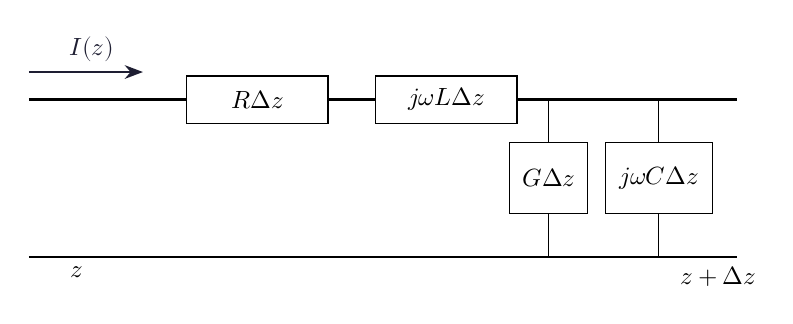
\begin{tikzpicture}[font=\small]
\draw[thick] (0,0)--(9,0) (0,2)--(2,2) (3.8,2)--(4.4,2) (6.2,2)--(9,2);
\draw (2,1.7) rectangle (3.8,2.3) node[pos=.5] {$R\Delta z$};
\draw (4.4,1.7) rectangle (6.2,2.3) node[pos=.5] {$j\omega L\Delta z$};
\draw (6.6,2)--(6.6,1.45) (6.6,.55)--(6.6,0) (8,2)--(8,1.45) (8,.55)--(8,0);
\draw (6.1,.55) rectangle (7.1,1.45) node[pos=.5] {$G\Delta z$};
\draw (7.32,.55) rectangle (8.68,1.45) node[pos=.5] {$j\omega C\Delta z$};
\draw[arrow] (0,2.35)--(1.45,2.35) node[above,pos=.55] {$I(z)$};
\node[below] at (.6,0) {$z$}; \node[below] at (8.75,0) {$z+\Delta z$};
\end{tikzpicture}
\end{tcolorbox}

Apply Kirchhoff's laws and take the limit:
\[
\begin{aligned}
V(z)-V(z+\Delta z)&=(R+j\omega L)\Delta z\,I(z),\\
I(z)-I(z+\Delta z)&\approx(G+j\omega C)\Delta z\,V(z),\\
\frac{dV}{dz}&=-Z'I,\qquad \frac{dI}{dz}=-Y'V ,
\end{aligned}
\]
where $Z'=R+j\omega L$ and $Y'=G+j\omega C$. The first equality is for the incremental circuit with its shunt at the right. The exact shunt voltage there is $V(z+\Delta z)$, replaced by $V(z)$ in the limit. The time-domain forms replace $j\omega$ by $\partial_t$ on the corresponding quantity.
\[
\begin{aligned}
V''&=Z'Y'V,\qquad I''=Z'Y'I,\\
V(z)&=V^+e^{-\gamma z}+V^-e^{\gamma z},\\
I(z)&=\frac{V^+}{Z_0}e^{-\gamma z}-\frac{V^-}{Z_0}e^{\gamma z}.
\end{aligned}
\]
Here $\gamma=\sqrt{Z'Y'}=\alpha+j\beta$ in $\mathrm{m^{-1}}$ and $Z_0=Z'/\gamma=\sqrt{Z'/Y'}$ in $\Omega$. Choose the passive forward branch. The minus sign in reflected current follows from $I=-V'/Z'$.
\begin{itemize}[leftmargin=*,itemsep=3pt]
\item \textbf{Lossless.} $R=G=0$, $Z_0=\sqrt{L/C}$, $\beta=\omega\sqrt{LC}$ and $v_p=1/\sqrt{LC}$.
\item \textbf{Low loss.} For $R\ll\omega L$ and $G\ll\omega C$, expand the square root to first order. Write $\gamma=j\omega\sqrt{LC}\sqrt{(1-jR/\omega L)(1-jG/\omega C)}$. With $\sqrt{1+x}\approx1+x/2$, $\alpha\approx R/(2Z_{00})+GZ_{00}/2$, $\beta\approx\omega\sqrt{LC}$ and $Z_{00}=\sqrt{L/C}$. The exact $Z_0$ may be complex.
\item \textbf{Distortionless case.} When $R/L=G/C$, $Z_0=\sqrt{L/C}$ and $\gamma=\sqrt{LC}(G/C+j\omega)$. Attenuation is independent of frequency and phase is linear under this ideal model.
\end{itemize}

\section{Termination, Impedance and Power}
\subsection{Reflection and standing waves}
Set load at $z=0$ and input at $z=-\ell$. At the load, $Z_L=Z_0(1+\Gamma_L)/(1-\Gamma_L)$ with $\Gamma_L=V^-/V^+$. Solve for $\Gamma_L$ and follow the phasors toward the generator:
\[
 \Gamma_L=\frac{Z_L-Z_0}{Z_L+Z_0},\qquad
 \Gamma_{\mathrm{in}}=\Gamma_L e^{-2\gamma\ell}.
\]
Short, open and matched loads give $-1$, $+1$ and 0 respectively. For a lossless line at distance $d$ from the load the relative phase is $\arg\Gamma_L-2\beta d$. Voltage maxima and minima occur when this is $0$ and $\pi$ modulo $2\pi$, respectively.
\begin{tcolorbox}[defbox,title={Voltage standing-wave ratio}]
The voltage standing-wave ratio (VSWR) is the voltage maximum divided by the voltage minimum. On a lossless line, $S=(1+|\Gamma_L|)/(1-|\Gamma_L|)$. Consecutive maxima are $\lambda/2$ apart and adjacent maximum and minimum are $\lambda/4$ apart. On appreciably lossy lines the ratio varies with position.
\end{tcolorbox}
\begin{tcolorbox}[examplebox,title={Complex load, VSWR and standing-wave positions}]
A lossless $50\,\Omega$ line ends in $Z_L=(75+j50)\,\Omega$. Distances $d$ are measured from the load toward the generator.
\[
\begin{aligned}
\Gamma_L&=\frac{25+j50}{125+j50}
  =\frac{(25+j50)(125-j50)}{125^2+50^2}\\
  &=0.3103+j0.2759=0.4152\angle41.6^\circ,\\
S&=\frac{1+0.4152}{1-0.4152}=2.42.
\end{aligned}
\]
For the nearest voltage maximum, $41.6^\circ-720^\circ d/\lambda=0$, so $d_{\max}=0.0578\lambda$. The first minimum is another $\lambda/4$ toward the generator, at $0.3078\lambda$. Use the magnitude of the reflection coefficient for VSWR and its phase for positions. About $82.8\%$ of the incident power reaches the load.
\end{tcolorbox}

\subsection{Exact and low-loss impedance transformation}
Substitute $\Gamma_{\mathrm{in}}$ into $Z_{\mathrm{in}}=Z_0(1+\Gamma_{\mathrm{in}})/(1-\Gamma_{\mathrm{in}})$, multiply numerator and denominator by $e^{\gamma\ell}(Z_L+Z_0)$ and group the exponential sums and differences. This gives
\[
 Z_{\mathrm{in}}=Z_0\frac{Z_L+Z_0\tanh(\gamma\ell)}{Z_0+Z_L\tanh(\gamma\ell)} .
\]
For lossless lines $\tanh(j\beta\ell)=j\tan\beta\ell$. For low-loss lines retain $\alpha\ell$ in the hyperbolic function if it is appreciable. Away from a pole, $\tanh(\alpha\ell+j\beta\ell)\approx j\tan\beta\ell+\alpha\ell\sec^2\beta\ell$ when the correction is small.
\begin{tcolorbox}[examplebox,title={Find characteristic impedance from open and short measurements}]
At the same frequency on the same uniform line section, measure the complex input impedances $Z_{\rm oc}$ and $Z_{\rm sc}$ by opening and shorting its far end. Taking $Z_L\to\infty$ and $Z_L=0$ gives
\[
\begin{aligned}
 Z_{\rm oc}&=Z_0\coth(\gamma\ell),&
 Z_{\rm sc}&=Z_0\tanh(\gamma\ell),\\
 Z_{\rm oc}Z_{\rm sc}&=Z_0^2 .
\end{aligned}
\]
Use the passive root. For $Z_{\rm sc}=j30\,\Omega$ and $Z_{\rm oc}=-j120\,\Omega$, $Z_0=60\,\Omega$. If the line is lossless and $0<\ell<\lambda/4$, then $\tan\beta\ell=30/60$ and $\ell/\lambda=\tan^{-1}(0.5)/(2\pi)=0.0738$ with the angle in radians.
\end{tcolorbox}

\begin{tcolorbox}[examplebox,title={Quarter-wave transformer and a low-loss comparison}]
To match a $100\,\Omega$ load to a $50\,\Omega$ feed, use a quarter-wave section with $Z_t=\sqrt{50(100)}=70.71\,\Omega$. Its lossless input is $Z_t^2/100=50\,\Omega$ at the design frequency.

For a $50\,\Omega$ line section itself feeding $100\,\Omega$, $\Gamma_L=1/3$. If $\ell=\lambda/4$ and $\alpha\ell=0.1$, take $Z_0\approx50\,\Omega$. Then $\Gamma_{\mathrm{in}}=-(1/3)e^{-0.2}=-0.2729$ and $Z_{\mathrm{in}}\approx28.56\,\Omega$. The lossless value is $25\,\Omega$.
\end{tcolorbox}
\subsection{Power transfer}
For peak phasors, $P=\operatorname{Re}(VI^*)/2$. At the load, use $V=V^++V^-$ and $I=(V^+-V^-)/Z_0$. For real $Z_0$ the product is
\[
 VI^*=\frac{|V^+|^2-|V^-|^2+
           V^-(V^+)^*-V^+(V^-)^*}{Z_0}.
\]
The two cross terms are a complex number minus its conjugate, so their real parts cancel. At the load this yields
\[
 P_L=\frac{|V^+|^2-|V^-|^2}{2Z_0}
 =\frac{|V^+|^2}{2Z_0}(1-|\Gamma_L|^2).
\]
Use $P_L/P_i=1-|\Gamma_L|^2$ and return loss $-20\log_{10}|\Gamma_L|$ in decibels. For complex $Z_0$ evaluate $\operatorname{Re}(VI^*)/2$ directly. Load matching removes reflection at that port. For maximum transfer from a fixed Thévenin generator, the load presented at the source reference plane must be the conjugate of its source impedance.
\begin{tcolorbox}[examplebox,title={Return loss, VSWR and delivered power}]
A $50\,\Omega$ lossless line delivers an incident $1\,\mathrm W$ to $Z_L=100\,\Omega$. $\Gamma_L=1/3$, $S=2$, return loss is $9.54\,\mathrm{dB}$ and $P_L=1(1-1/9)=0.889\,\mathrm W$.
\end{tcolorbox}

\section{Smith Chart and Matching}
\begin{tcolorbox}[defbox,title={Smith chart}]
A Smith chart maps normalized impedance to the complex voltage-reflection plane. Normalize $z_n=Z/Z_0=r+jx$ for a real $Z_0$. The centre is matched, the left rim is a short and the right rim an open.
\end{tcolorbox}
\subsection{Impedance and admittance grids}
For $\Gamma=u+jv$, use $z_n=(1+\Gamma)/(1-\Gamma)$. Taking real and imaginary parts and completing squares gives
\[
\begin{aligned}
 (u-r/(1+r))^2+v^2&=1/(1+r)^2,\\
 (u-1)^2+(v-1/x)^2&=1/x^2\qquad(x\ne0).
\end{aligned}
\]
Positive reactance lies above the real axis. The companion admittance grid is the impedance grid rotated by $180^\circ$ because $y_n=Y/Y_0=1/z_n$. On a single printed impedance grid, move to the diametrically opposite point to read the numerical $g+jb$. On a dual impedance/admittance chart, read the admittance grid at the original physical $\Gamma$ point. The change of grid alone is unrelated to line length.
\begin{tcolorbox}[tikzbox,title={Impedance Smith chart with a sample load},unbreakable]
\centering
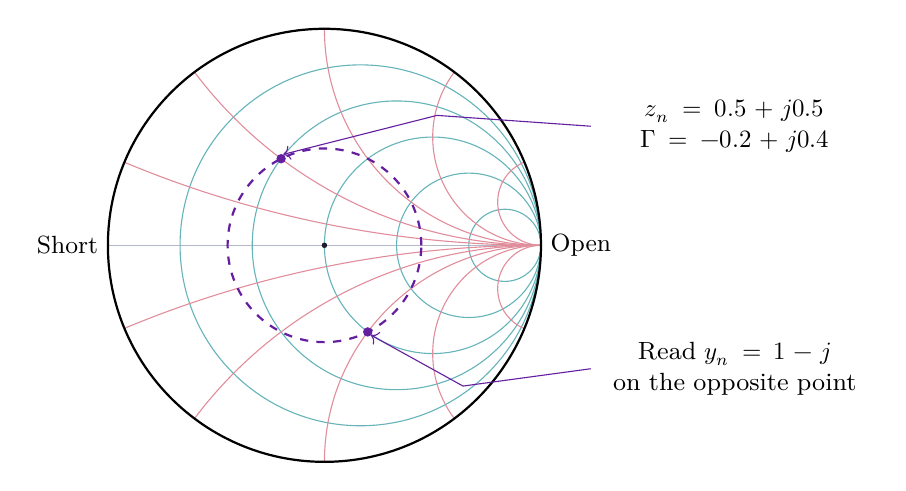
\begin{tikzpicture}[x=2.75cm,y=2.75cm,font=\small]
\begin{scope}
\clip (0,0) circle (1);
\draw[mgframe] (-1,0)--(1,0);
\foreach \r in {.2,.5,1,2,5}{
 \pgfmathsetmacro{\c}{\r/(1+\r)}
 \pgfmathsetmacro{\rad}{1/(1+\r)}
 \draw[myteal!60] (\c,0) circle (\rad);
}
\foreach \x in {.2,.5,1,2,5}{
 \pgfmathsetmacro{\rad}{1/\x}
 \draw[myred!50] (1,\rad) circle (\rad) (1,-\rad) circle (\rad);
}
\draw[dashed,mypurple,thick] (0,0) circle (.4472);
\end{scope}
\draw[thick] (0,0) circle (1);
\fill[mydark] (0,0) circle (1pt);
\fill[mypurple] (-.2,.4) circle (1.7pt) (.2,-.4) circle (1.7pt);
\node[align=center,text width=3.4cm,anchor=west] (load) at (1.23,.55) {$z_n=0.5+j0.5$\\$\Gamma=-0.2+j0.4$};
\draw[->,mypurple] (load.west)--(.52,.6)--(-.19,.42);
\node[align=center,text width=3.4cm,anchor=west] (adm) at (1.23,-.57) {Read $y_n=1-j$\\on the opposite point};
\draw[->,mypurple] (adm.west)--(.64,-.65)--(.215,-.415);
\node[left] at (-1,0) {Short}; \node[right] at (1,0) {Open};
\end{tikzpicture}
\end{tcolorbox}
\begin{enumerate}[leftmargin=*,itemsep=3pt]
\item Plot the normalized load at the intersection of its constant-$r$ circle and constant-$x$ arc.
\item Draw a constant-$|\Gamma|$ circle about the centre for a lossless line. Move clockwise toward the generator through $2\beta\ell$, or counterclockwise toward the load. A complete turn corresponds to $\lambda/2$.
\item Read the intersection with the new resistance and reactance curves. Multiply by $Z_0$ for ohms. With loss the point spirals inward on a generatorward move.
\item For $z_n=0.5+j0.5$ the illustrated point gives $|\Gamma|=\sqrt{0.2}$, so VSWR is $2.618$. A $\lambda/8$ move rotates clockwise by $90^\circ$, giving $\Gamma_{\mathrm{in}}=0.4+j0.2$ and $z_{\mathrm{in}}=2+j1$.
\end{enumerate}

\subsection{Single-stub matching and line sections as elements}
For a shunt stub, translate along the main line to a point with normalized admittance $1+jb$. Then add a stub of admittance $-jb$. An ideal stub carries reactive current and absorbs zero average power. Use the same real $Z_0$ for the main line and stub in the following example.
\begin{tcolorbox}[examplebox,title={Shunt shorted-stub match in admittance form}]
Take $Z_L=25\,\Omega$ on $Z_0=50\,\Omega$. Then $y_L=2$. At distance $d$ toward the generator, put $t=\tan\beta d$.
\[
 y(d)=\frac{2+jt}{1+j2t}
      =\frac{2(1+t^2)-j3t}{1+4t^2}.
\]
Set the real part to 1. This gives $t^2=1/2$. Choose $t=+0.7071$, hence $d=0.0980\lambda$, $y(d)=1-j0.7071$. A shorted stub gives $y_s=-j\cot(\beta\ell_s)$. Choose $\beta\ell_s=125.26^\circ$, or $\ell_s=0.3480\lambda$, so $y(d)+y_s=1$.
\end{tcolorbox}
\par\vspace{6pt}\noindent
\begin{tabularx}{\linewidth}{|B{4cm}|Y|}\hline
Lossless section & Input impedance or application \\ \hline
Short-circuit stub & $jZ_0\tan\beta\ell$. Electrically short: $j\omega L\ell$, an inductance. \\ \hline
Open-circuit stub & $-jZ_0\cot\beta\ell$. Electrically short: $1/(j\omega C\ell)$, a capacitance. \\ \hline
Quarter wavelength & $Z_0^2/Z_L$, so open and short exchange roles. A real load transforms through a suitable section impedance. \\ \hline
Half wavelength & Repeats $Z_L$ on a lossless line. Rotation on the Smith chart is a full turn. \\ \hline
\end{tabularx}


\newpage
\begin{center}
  {\large\bfseries\color{myred} Quick Revision --- Module 3}\\[3pt]
  {\small\color{mydark} Transmission Lines and Smith Chart $|$ EC501}
\end{center}
\noindent{\color{myred}\rule{\linewidth}{1.2pt}}
\begin{tcolorbox}[formulabox,title={Key Formulas at a Glance}]
\renewcommand{\arraystretch}{1.35}
\begin{tabularx}{\linewidth}{B{5.0cm}Y}
Distributed model & $\gamma=\sqrt{Z'Y'}$ and $Z_0=\sqrt{Z'/Y'}$ \\[3pt]
Voltage reflection & $\Gamma_L=(Z_L-Z_0)/(Z_L+Z_0)$ \\[3pt]
Input reflection & $\Gamma_{\mathrm{in}}=\Gamma_Le^{-2\gamma\ell}$ \\[3pt]
Standing-wave ratio & $(1+|\Gamma|)/(1-|\Gamma|)$ on a lossless line \\[3pt]
Real-impedance power & $P_L=P_i(1-|\Gamma_L|^2)$ for real $Z_0$ \\[3pt]
Quarter-wave match & $Z_t=\sqrt{Z_{\rm feed}R_L}$ for a resistive load \\[3pt]
\end{tabularx}
\end{tcolorbox}
\begin{tcolorbox}[defbox,title={One-Line Definitions}]
\textbf{Characteristic impedance.} Ratio of forward voltage to forward current on a uniform line.\par
\textbf{Reflection coefficient.} Complex ratio of reverse to forward voltage at a specified reference plane.\par
\textbf{Stub.} An open- or short-terminated section used as a frequency-dependent reactance or susceptance.\par
\end{tcolorbox}
\begin{tcolorbox}[exambox,title={Frequently Asked / Viva Questions}]
\begin{enumerate}[topsep=0pt, label=\textbf{Q\arabic*.}, itemsep=5pt]
\item \Q{What is the sign of reverse current?}
It is the negative of reverse voltage divided by $Z_0$ with current referenced toward the load.
\item \Q{When is a line lossless?}
When its series resistance and shunt conductance per metre are both zero.
\item \Q{How is a line's voltage equation obtained?}
Differentiate $V'=-Z'I$ and substitute $I'=-Y'V$.
\item \Q{What does matching at the load accomplish?}
It makes $\Gamma_L=0$.
\item \Q{What is the VSWR for an ideal open?}
Infinite on a lossless line because the voltage minimum is zero.
\item \Q{How far apart are adjacent voltage maxima?}
Half a wavelength.
\item \Q{Why does the load point rotate clockwise toward the generator?}
Its phase changes by $-2\beta\ell$.
\item \Q{How is admittance read on an impedance-only chart?}
Read the point diametrically opposite the normalized impedance.
\item \Q{What must the main-line admittance be for a shunt-stub match?}
Its normalized conductance must be one before stub susceptance cancels the imaginary part.
\item \Q{Why is a quarter-wave match frequency selective?}
The section has the required electrical length only at specified frequencies.
\end{enumerate}
\end{tcolorbox}
\begin{tcolorbox}[tikzbox,title={Summary comparison}]
\begin{tabularx}{\linewidth}{|B{4cm}|Y|}\hline
\textbf{Case} & \textbf{What to use} \\ \hline
Lossless movement & Clockwise along constant $|\Gamma|$ toward the generator. \\ \hline
Lossy movement & Clockwise and inward toward the generator. \\ \hline
Shunt stub & Match conductance first, then cancel susceptance. \\ \hline
\end{tabularx}
\end{tcolorbox}

% -- Module 4 -----------------------------------------------------------------
\modulestart{4}{Waveguide Modes and the General Method}

\section{Waveguide Modes and the General Method}
\begin{tcolorbox}[defbox,title={Mode and cutoff}]
A mode is a field distribution that satisfies Maxwell's equations and the guide boundaries. Cutoff is the frequency separating propagating from evanescent behaviour for that mode in an ideal uniform guide.
\end{tcolorbox}

Assume a homogeneous lossless fill, perfect electric conductor (PEC) walls, $e^{j\omega t}$ and longitudinal dependence $e^{-j\beta z}$. Set $k=\omega\sqrt{\mu\epsilon}$ and let $\nabla_t$ act in the cross-section only.
\par\vspace{6pt}\noindent
\begin{tabularx}{\linewidth}{|B{2.5cm}|Y|Y|}\hline
Mode & Longitudinal fields & Boundary condition on the metal walls \\ \hline
TEM & $E_z=H_z=0$ & Transverse potential is constant on each conductor. \\ \hline
TE & $E_z=0,\ H_z\ne0$ & $\partial H_z/\partial n=0$ for the transverse normal. \\ \hline
TM & $H_z=0,\ E_z\ne0$ & $E_z=0$ at the wall. \\ \hline
\end{tabularx}
\subsection{Solve longitudinal fields first}
\begin{enumerate}[leftmargin=*,itemsep=4pt]
\item Separate the wave equation using $\partial_z=-j\beta$. Both longitudinal fields satisfy $(\nabla_t^2+k_c^2)\Psi=0$, where $k_c^2=k^2-\beta^2$.
\item Find allowed $k_c$ from the PEC conditions. TM uses a zero-value condition because $E_z$ is tangential to a longitudinal wall. For TE, tangential electric field is proportional to $\partial_n H_z$, giving a zero-derivative condition.
\item Recover transverse fields for $k_c\ne0$. In the transverse curl equations, substitute $\partial_z=-j\beta$ and eliminate $\mathbf H_t$ or $\mathbf E_t$ to get
\[
\begin{aligned}
\mathbf E_t
 &=-\frac{j\beta}{k_c^2}\nabla_tE_z
   +\frac{j\omega\mu}{k_c^2}\hat{\mathbf z}\times\nabla_tH_z,\\
\mathbf H_t
 &=-\frac{j\beta}{k_c^2}\nabla_tH_z
   -\frac{j\omega\epsilon}{k_c^2}\hat{\mathbf z}\times\nabla_tE_z .
\end{aligned}
\]
For example, in TE, Faraday's transverse equation gives $\mathbf H_t=(\beta/\omega\mu)\hat{\mathbf z}\times\mathbf E_t$. Substitution into transverse Amp\`ere--Maxwell yields $k_c^2\mathbf E_t=j\omega\mu\,\hat{\mathbf z}\times\nabla_tH_z$.
\item Test the frequency. Above cutoff $\beta=\sqrt{k^2-k_c^2}$ is real. Below cutoff choose $\beta=-j\sqrt{k_c^2-k^2}$ so the field decays along $+z$.
\end{enumerate}
\subsection{Cutoff, guide wavelength and velocity}
With $v=1/\sqrt{\mu\epsilon}$ and $f_c=vk_c/(2\pi)$, define $s=\sqrt{1-(f_c/f)^2}$ above cutoff.
\[
\beta=ks,\qquad\lambda_g=\frac{2\pi}{\beta}=\frac{\lambda}{s},\qquad
v_p=\frac{v}{s},\qquad v_g=vs .
\]
Differentiate $\beta^2=\omega^2/v^2-k_c^2$ to get $d\beta/d\omega=\omega/(\beta v^2)$. This yields $v_g=v^2/v_p$. The phase speed may exceed $v$ while the group speed stays below it. The wave impedances are ratios of transverse field components with the forward-power orientation:
\[
Z_{\mathrm{TE}}=\frac{\omega\mu}{\beta}=\frac{\eta}{s},
\qquad Z_{\mathrm{TM}}=\frac{\beta}{\omega\epsilon}=\eta s.
\]

\section{Parallel-Plate Waveguide}
\begin{tcolorbox}[defbox,title={Parallel-plate waveguide}]
Two parallel conducting plates guide waves along their length. In the ideal model the plates are at $y=0$ and $y=d$ with fields invariant in $x$.
\end{tcolorbox}
\begin{itemize}[leftmargin=*,itemsep=3pt]
\item \textbf{TEM.} Equipotential plates give a linear transverse potential and a uniform electric field normal to the plates. Choose $\mathbf E=E_0\hat{\mathbf y}e^{-jkz}$ and $\mathbf H=-(E_0/\eta)\hat{\mathbf x}e^{-jkz}$ for forward power. There is no cutoff. For width $w\gg d$ with negligible fringing, $Z_0$ for plate voltage and total current is $\eta d/w$, distinct from $E/H=\eta$.
\item \textbf{TE.} $\partial_y H_z=0$ at both plates, hence $H_z=H_0\cos(m\pi y/d)$ with $m=1,2,\ldots$. The constant candidate gives no TE field.
\item \textbf{TM.} $E_z=0$ at both plates, hence $E_z=E_0\sin(m\pi y/d)$ with $m=1,2,\ldots$.
\item \textbf{Modal propagation.} In both higher-mode families $k_c=m\pi/d$ and $f_c=mv/(2d)$. Between zero and the first cutoff only TEM propagates.
\end{itemize}
\begin{tcolorbox}[tikzbox,title={Parallel plates carrying a TEM wave},unbreakable]
\centering
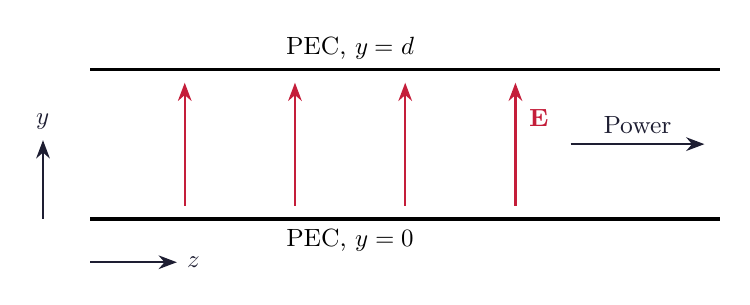
\begin{tikzpicture}[font=\small]
\draw[very thick] (0,0)--(8,0) (0,1.9)--(8,1.9);
\foreach \x in {1.2,2.6,4,5.4} \draw[redarrow] (\x,.17)--(\x,1.73);
\draw[arrow] (6.1,.95)--(7.8,.95) node[midway,above] {Power};
\draw[arrow] (0,-.55)--(1.1,-.55) node[right] {$z$};
\draw[arrow] (-.6,0)--(-.6,1) node[above] {$y$};
\node[above] at (3.3,1.9) {PEC, $y=d$};
\node[below] at (3.3,0) {PEC, $y=0$};
\node[right,myred] at (5.45,1.28) {$\mathbf E$};
\end{tikzpicture}
\end{tcolorbox}

\section{Rectangular Waveguide}
\subsection{Mode indices and dominant mode}
Let $a$ be the width in $x$ and $b$ the height in $y$. Separation in $x$ and $y$ gives $X''+k_x^2X=0$, $Y''+k_y^2Y=0$ and $k_x^2+k_y^2=k_c^2$. Enforcing the wall conditions gives
\[
\begin{aligned}
H_z&=H_0\cos(m\pi x/a)\cos(n\pi y/b)
 &&(\mathrm{TE},\ m,n\ge0,\ (m,n)\ne(0,0)),\\
E_z&=E_0\sin(m\pi x/a)\sin(n\pi y/b)
 &&(\mathrm{TM},\ m,n\ge1).
\end{aligned}
\]
Suppress the common $e^{-j\beta z}$ factor. Both families have
\[
 f_{c,mn}=\frac{v}{2}\sqrt{(m/a)^2+(n/b)^2}.
\]
For $a>b$, $\mathrm{TE}_{10}$ has the lowest cutoff $v/(2a)$ and is the dominant mode. The next cutoff is the smaller of $v/a$ ($\mathrm{TE}_{20}$) and $v/(2b)$ ($\mathrm{TE}_{01}$). Hollow single-conductor guide has no TEM mode. The transverse TEM potential would satisfy Laplace's equation with one constant value around the entire connected metal boundary. Uniqueness then forces a constant potential throughout and zero transverse electric field.
\subsection{Field visualization and surface current}
For $\mathrm{TE}_{10}$, let $k_x=\pi/a$ and drop the common axial factor. The only nonzero components are
\[
 H_z=H_0\cos(k_xx),\quad
 E_y=-\frac{j\omega\mu H_0}{k_x}\sin(k_xx),\quad
 H_x=\frac{j\beta H_0}{k_x}\sin(k_xx).
\]
At both side walls, tangential $E_y=0$ and $H_z$ is maximum in magnitude. Between these walls $|E_y|$ peaks at $a/2$. On the broad walls $E_y$ is normal, so its nonzero value is allowed and produces surface charge. There is no field variation across $y$ in this mode.
\begin{tcolorbox}[tikzbox,title={Electric field across the dominant-mode cross-section},unbreakable]
\centering
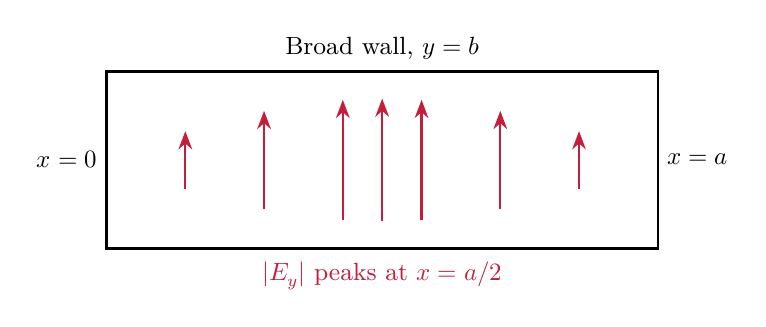
\begin{tikzpicture}[font=\small]
\draw[thick] (0,0) rectangle (7,2.25);
\foreach \x/\h in {1/.47,2/.8,3/.98,3.5/1,4/.98,5/.8,6/.47}
  \draw[redarrow] (\x,{1.125-.78*\h})--(\x,{1.125+.78*\h});
\node[above] at (3.5,2.28) {Broad wall, $y=b$};
\node[left] at (0,1.13) {$x=0$};
\node[right] at (7,1.13) {$x=a$};
\node[below,myred] at (3.5,-.04) {$|E_y|$ peaks at $x=a/2$};
\end{tikzpicture}
\end{tcolorbox}

For wall current, use the normal pointing from metal into guide and $\mathbf K=\hat{\mathbf n}\times\mathbf H$. At $x=0$, $\hat{\mathbf n}=\hat{\mathbf x}$ and $\mathbf K=-H_z\hat{\mathbf y}$. At $x=a$, $\hat{\mathbf n}=-\hat{\mathbf x}$ and $H_z=-H_0$, so $\mathbf K$ again points along $-\hat{\mathbf y}$ for the same $H_0$ phase. On the broad walls, the normal is $\pm\hat{\mathbf y}$. The wall current has both $x$ and $z$ components from $H_z$ and $H_x$, respectively. The current flows tangentially on all walls.

\subsection{Higher-mode field sketch and coupling}
For $\mathrm{TE}_{11}$ write $k_x=\pi/a$, $k_y=\pi/b$, $k_c^2=k_x^2+k_y^2$ and $H_z=H_0\cos(k_xx)\cos(k_yy)$. Use the TE transverse-field relation to get
\[
\begin{aligned}
 E_x &= \frac{j\omega\mu H_0 k_y}{k_c^2}\cos(k_xx)\sin(k_yy),\\
 E_y &=-\frac{j\omega\mu H_0 k_x}{k_c^2}\sin(k_xx)\cos(k_yy).
\end{aligned}
\]
To sketch, mark the midlines $x=a/2$ and $y=b/2$. On the $y$ midline only $E_x$ remains. On the $x$ midline only $E_y$ remains. All tangential electric components vanish at the PEC wall. Both components vanish at the centre of this particular mode.
\begin{tcolorbox}[tikzbox,title={TE11 cross-section at one field phase},unbreakable]
\centering
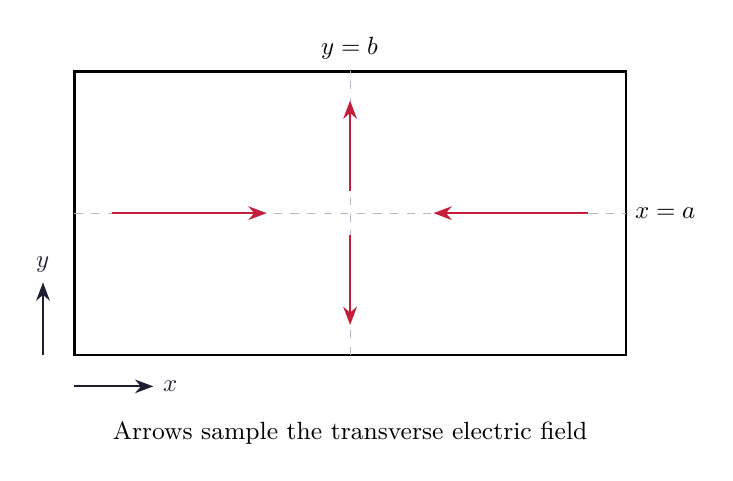
\begin{tikzpicture}[font=\small]
\draw[thick] (0,0) rectangle (7,3.6);
\draw[dashed,mgframe] (3.5,0)--(3.5,3.6) (0,1.8)--(7,1.8);
\draw[redarrow] (.48,1.8)--(2.44,1.8);
\draw[redarrow] (6.52,1.8)--(4.56,1.8);
\draw[redarrow] (3.5,1.52)--(3.5,.38);
\draw[redarrow] (3.5,2.08)--(3.5,3.23);
\draw[arrow] (0,-.4)--(1,-.4) node[right] {$x$};
\draw[arrow] (-.4,0)--(-.4,.92) node[above] {$y$};
\node[above] at (3.5,3.63) {$y=b$};
\node[right] at (7,1.8) {$x=a$};
\node[below] at (3.5,-.72) {Arrows sample the transverse electric field};
\end{tikzpicture}
\end{tcolorbox}

\textbf{Coupling out power.} An electric probe couples when it is placed at a nonzero electric field and aligned with that field. For example, a small $y$-directed probe at $x=a/2$, $y=b/4$ samples $E_y$ in $\mathrm{TE}_{11}$. A small loop instead couples to magnetic flux when its normal is aligned with the local magnetic field. Coupling also depends on which other modes are above cutoff and on how the coupler is matched.

\begin{tcolorbox}[examplebox,title={Cutoff ordering and below-cutoff decay}]
An air-filled guide has $a=30\,\mathrm{mm}$ and $b=15\,\mathrm{mm}$. The $\mathrm{TE}_{10}$ cutoff is $5\,\mathrm{GHz}$ and the $\mathrm{TE}_{20}$ and $\mathrm{TE}_{01}$ cutoffs are both $10\,\mathrm{GHz}$. The $\mathrm{TE}_{11}$ and $\mathrm{TM}_{11}$ cutoffs are both $\sqrt{5^2+10^2}=11.18\,\mathrm{GHz}$.

At $8\,\mathrm{GHz}$, only $\mathrm{TE}_{10}$ propagates. A semi-infinite guide's below-cutoff $\mathrm{TE}_{11}$ component decays with constant $\kappa=(2\pi/v)\sqrt{f_c^2-f^2}\approx164\,\mathrm{m^{-1}}$. At $20\,\mathrm{mm}$ the amplitude fraction is $e^{-\kappa(0.020)}\approx0.038$. This cutoff decay exists even with perfect walls. Ohmic attenuation above cutoff is a separate effect.
\end{tcolorbox}

\section{Guide Attenuation and Numerical Design}
\begin{tcolorbox}[defbox,title={Attenuation constant}]
If amplitude varies as $e^{-\alpha z}$, guided power varies as $e^{-2\alpha z}$. The amplitude attenuation is $\alpha$ in nepers per metre, or $8.686\alpha$ in decibels per metre.
\end{tcolorbox}
\begin{enumerate}[leftmargin=*,itemsep=4pt]
\item \textbf{Calculate transmitted power.} Use the ideal modal fields for small loss: $P=\tfrac12\operatorname{Re}\int_A(\mathbf E\times\mathbf H^*)\cdot\hat{\mathbf z}\,dA$.
\item \textbf{Calculate wall loss per metre.} The surface resistance is $R_s=\sqrt{\omega\mu_w/(2\sigma_w)}$ for a good metal. Integrate $P'_w=(R_s/2)\oint |\mathbf H_{\tan}|^2\,ds$ around the perimeter. Include both pairs of walls.
\item \textbf{Convert loss to attenuation.} Power balance gives $-dP/dz=P'_w=2\alpha_cP$, so $\alpha_c=P'_w/(2P)$.
\end{enumerate}
For $\mathrm{TE}_{10}$, integration of $\sin^2(k_xx)$ gives $a/2$. Thus $P=ab\,\omega\mu\beta |H_0|^2/(4k_x^2)$. The two side walls contribute $2b|H_0|^2$ to the perimeter integral. The broad walls contribute $a(1+\beta^2/k_x^2)|H_0|^2$. Substituting and using $q=f_c/f=k_x/k$ yields
\[
\alpha_c=\frac{R_s}{\eta b\sqrt{1-q^2}}\left[1+\frac{2b}{a}q^2\right].
\]
For a weakly lossy dielectric with loss tangent $\tan\delta_d$, replace $k^2$ by $k^2(1-j\tan\delta_d)$. Expanding the square root yields $\alpha_d\approx k^2\tan\delta_d/(2\beta)$. Add the two contributions when losses are small. Near cutoff, these perturbative estimates lose accuracy as $\beta\to0$.
\begin{tcolorbox}[examplebox,title={Single-mode test at 10 GHz}]
Take an air-filled guide $a=22.86\,\mathrm{mm}$, $b=10.16\,\mathrm{mm}$.
\begin{enumerate}[leftmargin=*,itemsep=2pt]
\item $f_{c,10}=6.56\,\mathrm{GHz}$, $f_{c,20}=13.12\,\mathrm{GHz}$, $f_{c,01}=14.76\,\mathrm{GHz}$. Only $\mathrm{TE}_{10}$ propagates at $10\,\mathrm{GHz}$.
\item With $\lambda=30.0\,\mathrm{mm}$ and $s=0.755$, $\lambda_g=39.7\,\mathrm{mm}$, $v_g=2.26\times10^8\,\mathrm{m/s}$ and $Z_{\mathrm{TE}}\approx499\,\Omega$.
\item For smooth copper with $R_s\approx0.0261\,\Omega$, $\alpha_c\approx0.0125\,\mathrm{Np/m}\approx0.109\,\mathrm{dB/m}$. Ideal air adds negligible dielectric loss.
\end{enumerate}
\end{tcolorbox}

\newpage
\begin{center}
  {\large\bfseries\color{myred} Quick Revision --- Module 4}\\[3pt]
  {\small\color{mydark} Parallel-Plate and Rectangular Waveguides $|$ EC501}
\end{center}
\noindent{\color{myred}\rule{\linewidth}{1.2pt}}
\begin{tcolorbox}[formulabox,title={Key Formulas at a Glance}]
\renewcommand{\arraystretch}{1.35}
\begin{tabularx}{\linewidth}{B{5.0cm}Y}
Dispersion relation & $\beta^2=k^2-k_c^2$ \\[3pt]
Plate cutoff & $f_c=mv/(2d)$ for higher modes \\[3pt]
Rectangular cutoff & $f_{c,mn}=(v/2)\sqrt{(m/a)^2+(n/b)^2}$ \\[3pt]
Guide wavelength & $\lambda_g=2\pi/\beta$ \\[3pt]
Wall current & $\mathbf K=\hat{\mathbf n}\times\mathbf H$ with metal-to-guide normal \\[3pt]
Amplitude attenuation & $\alpha_c=P'_w/(2P)$ \\[3pt]
\end{tabularx}
\end{tcolorbox}
\begin{tcolorbox}[defbox,title={One-Line Definitions}]
\textbf{Dominant mode.} Mode with the lowest cutoff frequency.\par
\textbf{Guide wavelength.} Distance along the guide giving a phase advance of one full cycle.\par
\textbf{Below-cutoff field.} Evanescent field that decays along the guide in a semi-infinite section.\par
\end{tcolorbox}
\begin{tcolorbox}[exambox,title={Frequently Asked / Viva Questions}]
\begin{enumerate}[topsep=0pt, label=\textbf{Q\arabic*.}, itemsep=5pt]
\item \Q{Why does a parallel-plate guide support TEM?}
Distinct conductors can be held at different transverse potentials.
\item \Q{Why does hollow rectangular guide lack TEM?}
Its single connected metal boundary forces a constant transverse potential.
\item \Q{Why can TE have one zero index?}
Cosine remains nonzero when one transverse index is zero.
\item \Q{Why cannot TM have a zero index?}
Its sine product vanishes identically.
\item \Q{What is dominant when the width exceeds the height?}
The $\mathrm{TE}_{10}$ mode.
\item \Q{What determines single-mode operation?}
Frequency lies above dominant cutoff and below the next allowed cutoff.
\item \Q{How do phase and group velocity compare?}
Above cutoff their product is $v^2$ for a nondispersive fill and ideal walls.
\item \Q{Where is the dominant-mode electric field largest?}
At $x=a/2$, directed across the guide height.
\item \Q{Which magnetic field determines wall loss?}
The field tangential to the metal.
\item \Q{Why is attenuation generally larger near cutoff?}
Modal power for a given field level drops as $\beta$ falls.
\end{enumerate}
\end{tcolorbox}
\begin{tcolorbox}[tikzbox,title={Summary comparison}]
\begin{tabularx}{\linewidth}{|B{4cm}|Y|}\hline
\textbf{Case} & \textbf{What to use} \\ \hline
TEM parallel plates & No cutoff. Both longitudinal components vanish. \\ \hline
TE rectangular & $H_z$ cosine product. One index may be zero. \\ \hline
TM rectangular & $E_z$ sine product. Both indices must be positive. \\ \hline
\end{tabularx}
\end{tcolorbox}

% -- Module 5 -----------------------------------------------------------------
\modulestart{5}{Electromagnetic Potentials and Radiation}

\section{Electromagnetic Potentials and Radiation}
\begin{tcolorbox}[defbox,title={Scalar and vector potentials}]
The vector potential $\mathbf A$ determines magnetic flux by $\mathbf B=\nabla\times\mathbf A$. The electric field is $\mathbf E=-\nabla\Phi-\partial_t\mathbf A$, where $\Phi$ is the scalar potential. Potentials are useful for finding the fields of localized charge and current distributions.
\end{tcolorbox}

Assume a uniform lossless medium, $v=1/\sqrt{\mu\epsilon}$, $k=\omega/v$, $\eta=\sqrt{\mu/\epsilon}$ and peak phasors with $e^{j\omega t}$. The potential representation satisfies magnetic Gauss law and Faraday's law. It allows the Lorenz gauge $\nabla\cdot\mathbf A=-j\omega\mu\epsilon\Phi$.
\subsection{Wave equations and their outgoing solutions}
Insert the potentials into Amp\`ere--Maxwell. Use $\nabla\times\nabla\times\mathbf A=\nabla(\nabla\cdot\mathbf A)-\nabla^2\mathbf A$:
\[
\begin{aligned}
\nabla(\nabla\cdot\mathbf A)-\nabla^2\mathbf A
 &=\mu\mathbf J-j\omega\mu\epsilon\nabla\Phi+k^2\mathbf A,\\
(\nabla^2+k^2)\mathbf A&=-\mu\mathbf J.
\end{aligned}
\]
Electric Gauss law gives $-\nabla^2\Phi-j\omega\nabla\cdot\mathbf A=\rho_v/\epsilon$, hence $(\nabla^2+k^2)\Phi=-\rho_v/\epsilon$. For an unbounded medium write $R=|\mathbf r-\mathbf r'|$:
\[
\begin{aligned}
\mathbf A(\mathbf r)&=\frac{\mu}{4\pi}\int_V
     \mathbf J(\mathbf r')\frac{e^{-jkR}}{R}\,dV',\\
\Phi(\mathbf r)&=\frac{1}{4\pi\epsilon}\int_V
     \rho_v(\mathbf r')\frac{e^{-jkR}}{R}\,dV'.
\end{aligned}
\]
Outside a point source the radial kernel solves the homogeneous Helmholtz equation. A small sphere about the source fixes the $1/(4\pi)$ factor by the flux integral. The outgoing sign follows because $\omega t-kR$ is a phase moving to larger $R$. In time domain each source is evaluated at the retarded time $t-R/v$.
\begin{itemize}[leftmargin=*,itemsep=3pt]
\item \textbf{Far-zone amplitude.} Use $1/R\approx1/r$ for $r$ much larger than the source size.
\item \textbf{Far-zone phase.} Keep $R\approx r-\hat{\mathbf r}\cdot\mathbf r'$ in the exponential. Discarding the second term can erase the directional pattern of an extended antenna.
\item \textbf{Field reconstruction.} The leading spatial derivative is $-jk\hat{\mathbf r}$. Thus $\mathbf H_{\rm far}\approx-jk\hat{\mathbf r}\times\mathbf A/\mu$ and $\mathbf E_{\rm far}\approx\eta\mathbf H_{\rm far}\times\hat{\mathbf r}$.
\end{itemize}

\section{Hertzian Dipole}
\begin{tcolorbox}[defbox,title={Hertzian dipole}]
A Hertzian dipole is an ideal electrically short current element of length $\ell\ll\lambda$, carrying uniform peak phasor current $I_0$. Its moment $I_0\ell$ is directed along the element.
\end{tcolorbox}

For an element at the origin along $z$, $\mathbf A=\hat{\mathbf z}\mu I_0\ell e^{-jkr}/(4\pi r)$. Use $\hat{\mathbf z}=\hat{\mathbf r}\cos\theta-\hat{\boldsymbol\theta}\sin\theta$.
\[
H_\phi=\frac{\partial_r(r A_\theta)-\partial_\theta A_r}{\mu r}
  =\frac{I_0\ell\sin\theta}{4\pi}e^{-jkr}
   \left(\frac{jk}{r}+\frac{1}{r^2}\right).
\]
Outside the source, $\mathbf E=(\nabla\times\mathbf H)/(j\omega\epsilon)$. Define $C=I_0\ell e^{-jkr}/(4\pi)$ at the field point. The nonzero electric components are
\[
\begin{aligned}
E_r&=2\eta C\cos\theta\left(\frac{1}{r^2}+\frac{1}{jk r^3}\right),\\
E_\theta&=\eta C\sin\theta\left(\frac{jk}{r}+\frac{1}{r^2}+\frac{1}{jk r^3}\right).
\end{aligned}
\]
The $1/r^3$ and $1/r^2$ terms matter in the near field. At $kr\gg1$ keep only $1/r$ terms: $E_\theta\approx\eta H_\phi=j\eta k I_0\ell\,e^{-jkr}\sin\theta/(4\pi r)$. The fields are transverse and in phase, with outward mean power. The axial direction is a null and broadside is maximum. The field is linearly polarized along $\hat{\boldsymbol\theta}$ away from nulls.
\begin{tcolorbox}[tikzbox,title={Hertzian dipole and normalized elevation-plane power pattern},unbreakable]
\centering
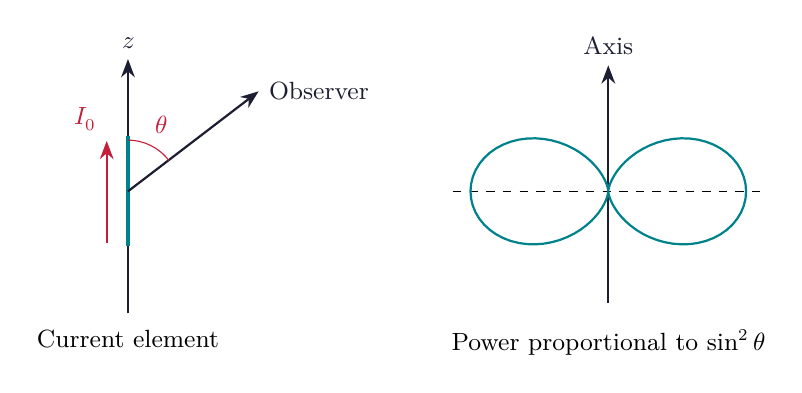
\begin{tikzpicture}[font=\small]
\draw[arrow] (0,-1.55)--(0,1.68) node[above] {$z$};
\draw[very thick,myteal] (0,-.7)--(0,.7);
\draw[redarrow] (-.27,-.66)--(-.27,.64) node[above left] {$I_0$};
\draw[arrow] (0,0)--(1.66,1.27) node[right] {Observer};
\draw[myred] (0,.65) arc (90:37:.65);
\node[myred] at (.42,.85) {$\theta$};
\node[below] at (0,-1.63) {Current element};
\begin{scope}[xshift=6.1cm]
\draw[arrow] (0,-1.42)--(0,1.6) node[above] {Axis};
\draw[dashed] (-1.97,0)--(1.97,0);
\draw[thick,myteal,domain=0:360,samples=121]
 plot ({1.75*sin(\x)^3},{1.75*sin(\x)^2*cos(\x)});
\node[below] at (0,-1.63) {Power proportional to $\sin^2\theta$};
\end{scope}
\end{tikzpicture}
\end{tcolorbox}
\subsection{Radiated power and radiation resistance}
Radiation intensity $U=r^2\langle S_r\rangle$ is power per solid angle, in $\mathrm{W/sr}$. In the radiation zone $\langle S_r\rangle=|E_\theta|^2/(2\eta)$. Integrate over a sphere:
\[
\begin{aligned}
U(\theta)&=\frac{\eta k^2|I_0\ell|^2}{32\pi^2}\sin^2\theta,\\
P_{\rm rad}&=\frac{\eta k^2|I_0\ell|^2}{32\pi^2}
 \int_0^{2\pi}d\phi\int_0^\pi\sin^3\theta\,d\theta\\
 &=\frac{\eta k^2|I_0\ell|^2}{12\pi}.
\end{aligned}
\]
The last integral is $4/3$ by substitution $u=\cos\theta$. With peak current $P_{\rm rad}=|I_0|^2R_r/2$, so $R_r=\eta k^2\ell^2/(6\pi)=80\pi^2(\ell/\lambda)^2\,\Omega$ in free space. Finally $D_0=4\pi U_{\max}/P_{\rm rad}=1.5=1.76\,\mathrm{dBi}$.
\begin{tcolorbox}[examplebox,title={Power from a current element}]
In free space, take $\ell=\lambda/20$ and $I_0=2\,\mathrm A$ peak. Then $R_r=80\pi^2/400=1.974\,\Omega$ and $P_{\rm rad}=(2^2/2)(1.974)=3.95\,\mathrm W$. The result is for uniform current. A physical short dipole of the same length with triangular current radiates less for the same feed current.
\end{tcolorbox}

\section{Antenna Parameters and Reception}
\begin{tcolorbox}[defbox,title={Radiation pattern and antenna gain}]
A radiation pattern describes directional variation of far field or power. Directivity compares radiation intensity with the average intensity over the sphere. Gain also accounts for power dissipated within the antenna.
\end{tcolorbox}
\subsection{Pattern, power and feed quantities}
\par\vspace{6pt}\noindent
\begin{tabularx}{\linewidth}{|B{3.9cm}|Y|}\hline
Parameter & Definition or formula \\ \hline
Directivity & $D(\theta,\phi)=4\pi U/P_{\rm rad}$. $D_0$ is its maximum. \\ \hline
Radiation efficiency and gain & $e_r=P_{\rm rad}/P_{\rm accepted}$ and $G=e_rD$. Realized gain further includes mismatch at the chosen port. \\ \hline
Beamwidth & Half-power beamwidth (HPBW) is the angle between the two $-3\,\mathrm{dB}$ points around a lobe. First-null beamwidth is the angle between the first nulls where both exist in that cut. \\ \hline
Input impedance & $Z_A=R_r+R_{\rm loss}+jX_A$. Resonance means $X_A=0$, while feed matching also depends on the real part. \\ \hline
Bandwidth & Frequency interval satisfying a stated criterion, such as acceptable voltage standing-wave ratio, gain or pattern. Fractional bandwidth is $(f_H-f_L)/f_0$. \\ \hline
Polarization & Direction and time trajectory of the far electric vector for a specified observation direction. \\ \hline
\end{tabularx}

For a Hertzian dipole, $\sin^2\theta=1/2$ at $45^\circ$ and $135^\circ$. Thus the elevation HPBW is $90^\circ$. The azimuth cut at $\theta=90^\circ$ is omnidirectional.
\begin{tcolorbox}[examplebox,title={Separate directivity, gain and realized gain}]
Suppose $U_{\max}=0.40\,\mathrm{W/sr}$, $P_{\rm rad}=2\,\mathrm W$ and $P_{\rm accepted}=2.5\,\mathrm W$. At the specified feed plane $|\Gamma|=0.30$.
\[
\begin{aligned}
D_0&=4\pi(0.40)/2=2.51,& e_r&=2/2.5=0.80,\\
G_0&=0.80(2.51)=2.01,& G_{\rm realized}&=(1-0.30^2)(2.01)=1.83 .
\end{aligned}
\]
The gains are linear ratios. Apply $10\log_{10}$ to obtain $3.03\,\mathrm{dBi}$ for gain and $2.62\,\mathrm{dBi}$ for realized gain. The latter uses incident feed power before mismatch.
\end{tcolorbox}

\subsection{Receiving antenna and effective aperture}
\begin{itemize}[leftmargin=*,itemsep=3pt]
\item \textbf{Receive model.} For a reciprocal antenna, transmit and receive directional patterns agree. An incident wave induces an open-circuit voltage at the antenna terminals. For aligned linear polarization write $V_{\rm oc}=E_{\rm inc}h_{\rm eff}$, where effective length $h_{\rm eff}$ is measured in metres.
\item \textbf{Maximum available power.} Model the antenna as a Th\'evenin source $V_{\rm oc}$ in series with $Z_A=R_A+jX_A$. With load $Z_A^*$ the current magnitude is $|V_{\rm oc}|/(2R_A)$. This gives $P_{\rm av}=|V_{\rm oc}|^2/(8R_A)$ for peak voltage.
\item \textbf{Effective aperture.} $A_e=P_{\rm av}/S_{\rm inc}$ for polarization match. With $S_{\rm inc}=|E_{\rm inc}|^2/(2\eta)$, the aligned effective length result gives $A_e=\eta|h_{\rm eff}|^2/(4R_A)$. The reciprocal gain relation is $A_e=\lambda^2G/(4\pi)$, in $\mathrm{m^2}$ for gain in the arrival direction.
\item \textbf{Polarization mismatch.} Multiply by the squared magnitude of the overlap of unit polarization vectors. For linear polarizations tilted by $\psi$ this is $\cos^2\psi$.
\end{itemize}
\begin{tcolorbox}[examplebox,title={Friis relation and received power}]
In free-space far-field propagation, flux at range $R$ is $P_t G_t/(4\pi R^2)$ for accepted transmitter power $P_t$. Multiply by $A_e$ to get $P_r=P_tG_tG_r(\lambda/(4\pi R))^2$ for alignment and conjugate match. At $\lambda=0.30\,\mathrm m$, $R=100\,\mathrm m$, $P_t=1\,\mathrm W$, and $G_t=G_r=2$ (linear),
\[
 A_e=\frac{0.30^2(2)}{4\pi}=0.0143\,\mathrm{m^2},
 \qquad P_r\approx2.28\times10^{-7}\,\mathrm W.
\]
A $45^\circ$ linear polarization mismatch halves this received power.
\end{tcolorbox}

\section{Practical Dipoles and Monopoles}
\begin{tcolorbox}[defbox,title={Dipole and monopole}]
A centre-fed dipole has two conducting arms, one on each side of the feed. A monopole uses one arm and a conducting ground reference, with return current on the ground structure.
\end{tcolorbox}
\subsection{Short and half-wave dipoles}
\begin{itemize}[leftmargin=*,itemsep=3pt]
\item \textbf{Short practical dipole.} Current drops approximately linearly from $I_0$ at the centre to zero at the tips. The integral of the triangular profile is $I_0\ell/2$. Thus the far field is half the uniform-element result and $R_r\approx20\pi^2(\ell/\lambda)^2\,\Omega$ in free space.
\item \textbf{Half-wave thin dipole.} For total length $\lambda/2$, the approximate current is $I(z')=I_0\cos(kz')$ for $|z'|\le\lambda/4$. The element projection gives a $\sin\theta$ factor in $E_\theta$.
\end{itemize}
For the half-wave case define $u=\cos\theta$. The phase integral is even after dropping its odd part:
\[
 \int_{-\lambda/4}^{\lambda/4}\cos(kz')e^{jkuz'}\,dz'
   =\frac{2\cos(\pi u/2)}{k(1-u^2)}.
\]
To evaluate it, use $2\cos(kz')\cos(kuz')=\cos[k(1-u)z']+\cos[k(1+u)z']$. Multiplication by $\sin\theta$ gives the normalized field pattern $\cos[(\pi/2)\cos\theta]/\sin\theta$. Its limiting axial value is zero. The thin half-wave model gives approximately $73\,\Omega$ radiation resistance and $D_0\approx1.64$ ($2.15\,\mathrm{dBi}$). An exactly half-wavelength thin dipole has residual reactance. A slightly shorter length is commonly used for resonance, depending on diameter and surroundings.
\subsection{Quarter-wave monopole and image theory}
An ideal vertical quarter-wave monopole over an infinite perfect conducting plane has an in-phase vertical image. The upper-half-space field matches that of a half-wave dipole with the same feed current. The ground enforces zero tangential electric field and excludes radiation into the lower half-space.
\begin{tcolorbox}[tikzbox,title={Quarter-wave monopole and its image},unbreakable]
\centering
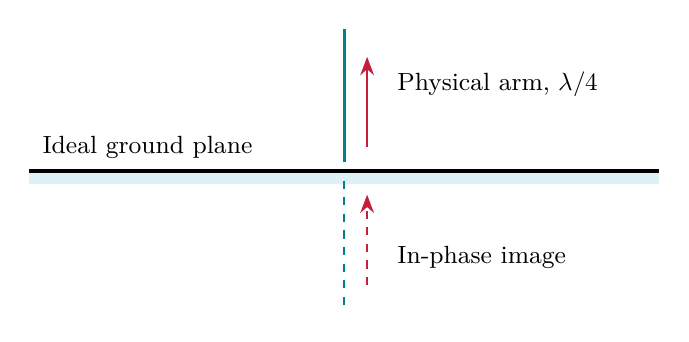
\begin{tikzpicture}[font=\small]
\fill[hdrteal] (-4,-.16) rectangle (4,0);
\draw[very thick] (-4,0)--(4,0);
\draw[very thick,myteal] (0,.12)--(0,1.8);
\draw[thick,myteal,dashed] (0,-.12)--(0,-1.8);
\draw[redarrow] (.29,.3)--(.29,1.45);
\draw[redarrow,dashed] (.29,-1.45)--(.29,-.3);
\node[right] at (.55,1.1) {Physical arm, $\lambda/4$};
\node[right] at (.55,-1.1) {In-phase image};
\node[above] at (-2.5,.03) {Ideal ground plane};
\end{tikzpicture}
\end{tcolorbox}
\begin{itemize}[leftmargin=*,itemsep=3pt]
\item \textbf{Power and resistance.} Same upper field at the same feed current, but half the total radiated power. Hence $R_r\approx36.5\,\Omega$.
\item \textbf{Directivity.} Maximum intensity stays the same while total power halves, so $D_0\approx3.28$ ($5.15\,\mathrm{dBi}$), referenced to a full sphere.
\item \textbf{Applications and limits.} Dipoles can give simple balanced antennas. Monopoles are compact over conductive bodies or radial ground systems. Finite ground, losses and surroundings change impedance and pattern.
\end{itemize}
At $600\,\mathrm{MHz}$ in free space, $\lambda=c/f=0.50\,\mathrm m$. The half-wave dipole is $0.25\,\mathrm m$ end to end with two $0.125\,\mathrm m$ arms. A quarter-wave monopole has one $0.125\,\mathrm m$ arm above ground. Practical tuning adjusts these first estimates.

\section{Past-Paper Extension: Folded Dipole and Arrays}
These applications appeared in a \href{https://www.scribd.com/document/972492704/Electromagnetic-Waves-EC501-5587-I040}{2022--23 EC501 paper} and extend the named topics in Module 5.
\subsection{Folded half-wave dipole}
\begin{tcolorbox}[defbox,title={Folded dipole}]
A folded dipole uses two closely spaced parallel conductors joined at both ends. One conductor is split at its centre for the balanced feed. Its overall span is approximately $\lambda/2$.
\end{tcolorbox}
\begin{tcolorbox}[tikzbox,title={Folded dipole and its in-phase radiation currents},unbreakable]
\centering
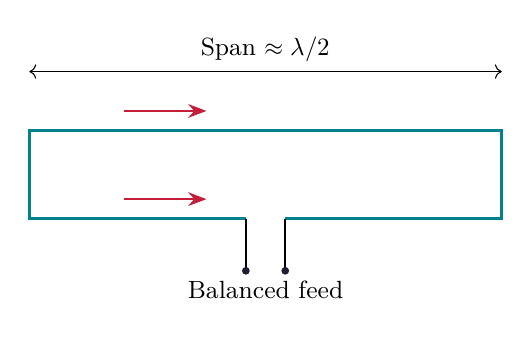
\begin{tikzpicture}[font=\small]
\draw[very thick,myteal] (-.25,0)--(-3,0)--(-3,1.12)--(3,1.12)--(3,0)--(.25,0);
\draw[thick] (-.25,0)--(-.25,-.66) (.25,0)--(.25,-.66);
\fill[mydark] (-.25,-.66) circle (1.4pt) (.25,-.66) circle (1.4pt);
\draw[redarrow] (-1.8,.25)--(-.75,.25);
\draw[redarrow] (-1.8,1.37)--(-.75,1.37);
\node[below] at (0,-.67) {Balanced feed};
\draw[<->] (-3,1.87)--(3,1.87) node[midway,above] {Span $\approx\lambda/2$};
\end{tikzpicture}
\end{tcolorbox}

\begin{enumerate}[leftmargin=*,itemsep=4pt]
\item \textbf{Current and pattern.} For small spacing and equal wire diameters, the in-phase radiation currents have approximately equal half-wave profiles, largest near the centre. Their fields add to give nearly the same normalized pattern as an ordinary half-wave dipole.
\item \textbf{Input resistance.} Near resonance, the folded antenna radiates approximately as an ordinary dipole carrying twice the folded antenna's feed current. At feed current $I$, equate $\tfrac12|I|^2R_{\rm folded}$ with $\tfrac12|2I|^2R_r$. Thus $R_{\rm folded}\approx4R_r\approx292\,\Omega$, often quoted as about $300\,\Omega$. The estimate assumes equal wire diameters, close spacing and negligible loss.
\item \textbf{Bandwidth.} The two-conductor structure alters the input impedance versus frequency and can give a wider usable matching band than a thin single-wire dipole. Actual bandwidth depends on spacing, wire diameter and the VSWR limit.
\end{enumerate}

\subsection{Array factor, broadside and end-fire}
\begin{tcolorbox}[defbox,title={Antenna array}]
An antenna array uses multiple elements whose fields combine in space. Relative excitation amplitudes and phases control the beam direction, beamwidth and sidelobes.
\end{tcolorbox}

Take two identical equally oriented elements at $0$ and $d\hat{\mathbf z}$, each carrying the same current magnitude, with feed phase advance $\delta$ on the second element. Neglect mutual coupling for this pattern calculation. In direction $\theta$ from the array axis the second path is shorter by $d\cos\theta$. With the outgoing phase convention,
\[
\psi=kd\cos\theta+\delta,\qquad
AF=1+e^{j\psi}=2e^{j\psi/2}\cos(\psi/2).
\]
Multiply the element field pattern by $AF$. Power varies as the squared magnitude of the product. With $d=\lambda/4$ and $\delta=0$, the array-factor maximum is at $\theta=90^\circ$ (broadside). With $\delta=-\pi/2$, its maximum occurs at $\theta=0^\circ$ ($+z$ end-fire) and its null is at $\theta=180^\circ$. The element pattern must also permit radiation in the chosen direction.
\begin{itemize}[leftmargin=*,itemsep=3pt]
\item \textbf{Linear array.} Elements lie on a line. A progressive phase controls the beam angle relative to the line.
\item \textbf{Planar and circular arrays.} A planar grid can steer in two angular coordinates. A circular arrangement provides azimuthal symmetry in the geometry and can steer in azimuth.
\item \textbf{Driven and parasitic elements.} Driven elements have a feed. Parasitic elements obtain current by coupling, as in the reflector and directors of a Yagi--Uda antenna.
\end{itemize}

\newpage
\begin{center}
  {\large\bfseries\color{myred} Quick Revision --- Module 5}\\[3pt]
  {\small\color{mydark} Radiation and Antennas $|$ EC501}
\end{center}
\noindent{\color{myred}\rule{\linewidth}{1.2pt}}
\begin{tcolorbox}[formulabox,title={Key Formulas at a Glance}]
\renewcommand{\arraystretch}{1.35}
\begin{tabularx}{\linewidth}{B{5.0cm}Y}
Outgoing kernel & $e^{-jkR}/(4\pi R)$ for time dependence $e^{j\omega t}$ \\[3pt]
Hertzian far field & $E_\theta\approx j\eta k I_0\ell\,e^{-jkr}\sin\theta/(4\pi r)$ \\[3pt]
Radiated power & $\int U\,d\Omega=\eta k^2|I_0\ell|^2/(12\pi)$ for a current element \\[3pt]
Directivity and gain & $D=4\pi U/P_{\rm rad}$, $G=e_r D$ \\[3pt]
Effective aperture & $A_e=\lambda^2G/(4\pi)$ under receive match \\[3pt]
Free-space link & $P_r/P_t=G_tG_r(\lambda/(4\pi R))^2$ for aligned matched link \\[3pt]
\end{tabularx}
\end{tcolorbox}
\begin{tcolorbox}[defbox,title={One-Line Definitions}]
\textbf{Radiation resistance.} Equivalent feed resistance that accounts for power radiated at the specified current.\par
\textbf{Effective aperture.} Available received power divided by incident power flux density for matched polarization.\par
\textbf{Radiation intensity.} Far-zone power radiated per unit solid angle.\par
\end{tcolorbox}
\begin{tcolorbox}[exambox,title={Frequently Asked / Viva Questions}]
\begin{enumerate}[topsep=0pt, label=\textbf{Q\arabic*.}, itemsep=5pt]
\item \Q{Why does the outgoing kernel use a negative phase exponent?}
With $e^{j\omega t}$ it gives a phase moving outward as time increases.
\item \Q{Why keep a position-dependent phase within the source?}
Phase differences between source elements determine the directional far-field pattern.
\item \Q{Which far-field terms carry power to large range?}
The transverse $1/r$ fields supply flux proportional to $1/r^2$.
\item \Q{Where is a Hertzian dipole's pattern null?}
In both directions along its axis.
\item \Q{Why are gain and directivity different?}
Gain includes radiation efficiency.
\item \Q{How does receive polarization tilt affect power?}
Linear tilt by $\psi$ multiplies matched received power by $\cos^2\psi$.
\item \Q{What load maximizes power from a receiving antenna?}
The complex conjugate of its input impedance in the Th\'evenin model.
\item \Q{Why is practical short-dipole radiation resistance smaller?}
Triangular current gives half the current moment of a uniform element at the same feed current and length.
\item \Q{What is the approximate thin half-wave dipole radiation resistance?}
About $73\,\Omega$ in free space.
\item \Q{Why does a quarter-wave monopole have half that resistance?}
At the same current it reproduces the dipole field in half the space and radiates half the total power.
\item \Q{What is the approximate resistance of an equal-wire folded dipole near resonance?}
About $300\,\Omega$, roughly four times that of an ordinary half-wave dipole.
\item \Q{Where do broadside and end-fire arrays point?}
Broadside points perpendicular to the array axis, while end-fire points along it.
\end{enumerate}
\end{tcolorbox}
\begin{tcolorbox}[tikzbox,title={Summary comparison}]
\begin{tabularx}{\linewidth}{|B{4cm}|Y|}\hline
\textbf{Case} & \textbf{What to use} \\ \hline
Hertzian element & Uniform current. Free-space directivity $1.5$. \\ \hline
Half-wave dipole & Approximate sinusoidal current. Directivity $1.64$. \\ \hline
Quarter-wave monopole & Image equivalence over ideal ground. Directivity $3.28$. \\ \hline
\end{tabularx}
\end{tcolorbox}

\end{document}
